\documentclass[aspectratio=169,xcolor=dvipsnames]{beamer}
\usetheme{SimpleDarkBlue}
\usepackage{hyperref}
\usepackage{graphicx} % Allows including images
\usepackage{booktabs} % Allows the use of \toprule, \midrule and \bottomrule in tables
\usepackage[spanish]{babel}
\usepackage[utf8]{inputenc}
\usepackage{array}
\usepackage{tabularx}
\usepackage{caption}
\usepackage{adjustbox}
\graphicspath{{graficas/graficas_presentacion/}}

\title{Construcción y optimización de un portafolio que replique el IPC S\&P/BMV mediante clustering y programación entera}
\subtitle{Replicación del índice de precios y cotizaciones de la bola mexicana de valores}

\author{Práxedis Jiménez Ruvalcaba, Jonathan Raymundo Torres Cárdenas \\ Asesor: M.A. Beatriz Alejandra García Ramos \\ }

\institute
{
    Facultad de Ciencias Físico Matemáticas \\
    Universidad Áutónoma de Nuevo León
}
\date{\today}

\begin{document}

\begin{frame}[c]
    \begin{beamercolorbox}[sep=8pt,center,rounded=true,shadow=true]{title}
        \usebeamerfont{title}\inserttitle\par
        \ifx\insertsubtitle\@empty
        \else
          \vskip0.25em
          {\usebeamerfont{subtitle}\insertsubtitle\par}
        \fi 
    \end{beamercolorbox}

    \vspace{1cm}
    \begin{center}
        \usebeamerfont{author}\insertauthor\par
        \vspace{0.5cm}
        \usebeamerfont{institute}\insertinstitute\par
        \usebeamerfont{date}\insertdate
    \end{center}
    
\end{frame}

\section{Objetivo, justificación y motivación}
\begin{frame}{Objetivo}
    \quad utilizar una combinación de técnicas de clustering y programación entera para construir un portafolio que 
    replique el índice de precios y cotizaciones (IPC) S\&P/BMV. Para posteriormente evaluar su optimización mediante
    la \textit{Modern Portfolio Theory} de Harry Markowitz (1952)\footnote{Markowitz, H. (1952). \emph{Portfolio selection}.
    JSTOR. (pp 77- 91).}, con el objetivo de analizar si este modelo estándar resulta suficiente bajo las condiciones del
    mercado nacional o si, por el contrario, es necesario desarrollar enfoques alternativos más adecuados para la realidad mexicana. 
\end{frame}

\begin{frame}{Justificación y motivación}
    \begin{itemize}
        \item Es común hallar trabajos en economía que toman datos de países alejados de la realidad nacional,
        por lo que sus resultados también distan de nuestro contexto.
        \item La \textit{modern portfolio theory} cuenta con muchas limitantes, aún así este es un estándar.
        \item Existe un valor en adaptar otros trabajos, para ver si es aplicable a nuestra realidad y si no, ampliarlo en otros contextos.
    \end{itemize}
\end{frame}

\begin{frame}{Justificación y motivación: Composición de índices}
    \begin{figure}[htp]
    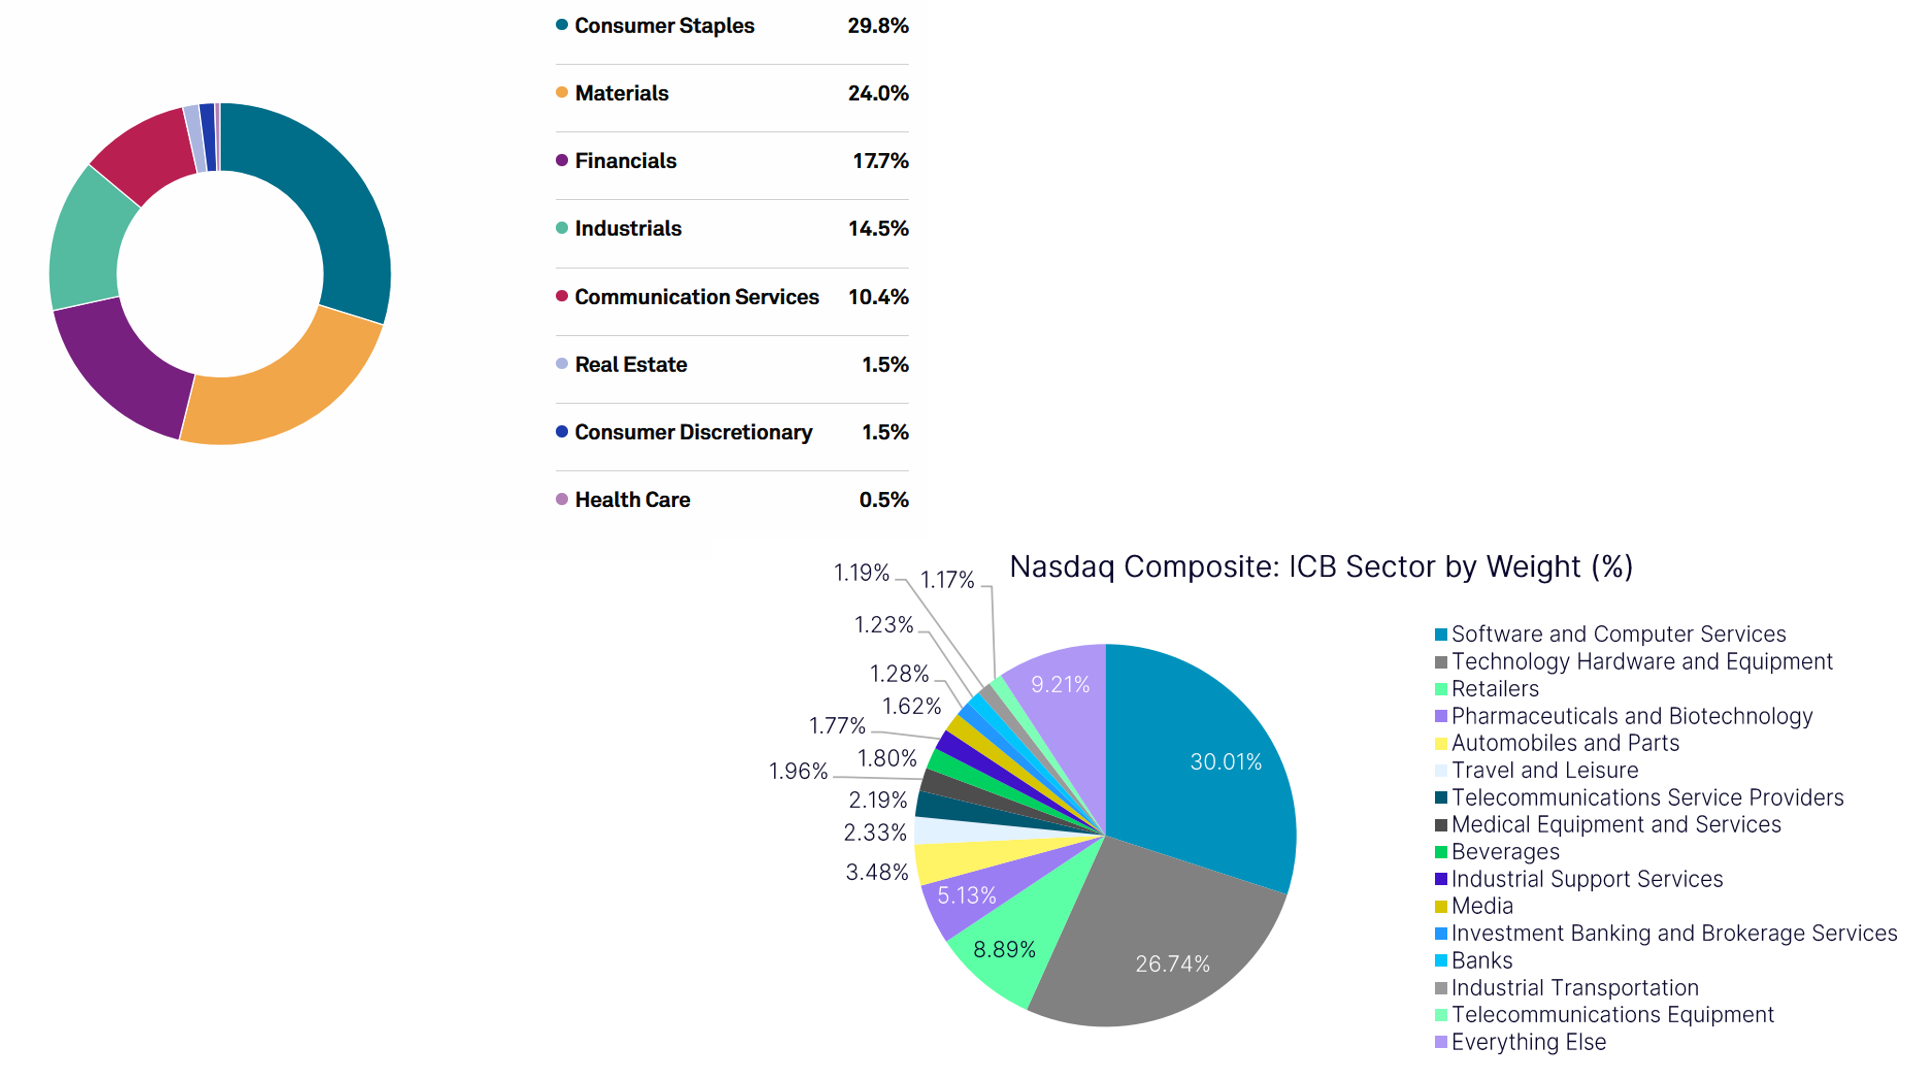
\includegraphics[width=8cm]{Composicion indice.png}
    \caption{Distribución por sector del IPC S\&P/BMV (arriba izq.) y del NASDAQ100 (abajo der.)}
    \end{figure}
\end{frame}

\begin{frame}{Justificación y motivación: Diferencias en comportamiento de índices}
    \begin{figure}[htp]
    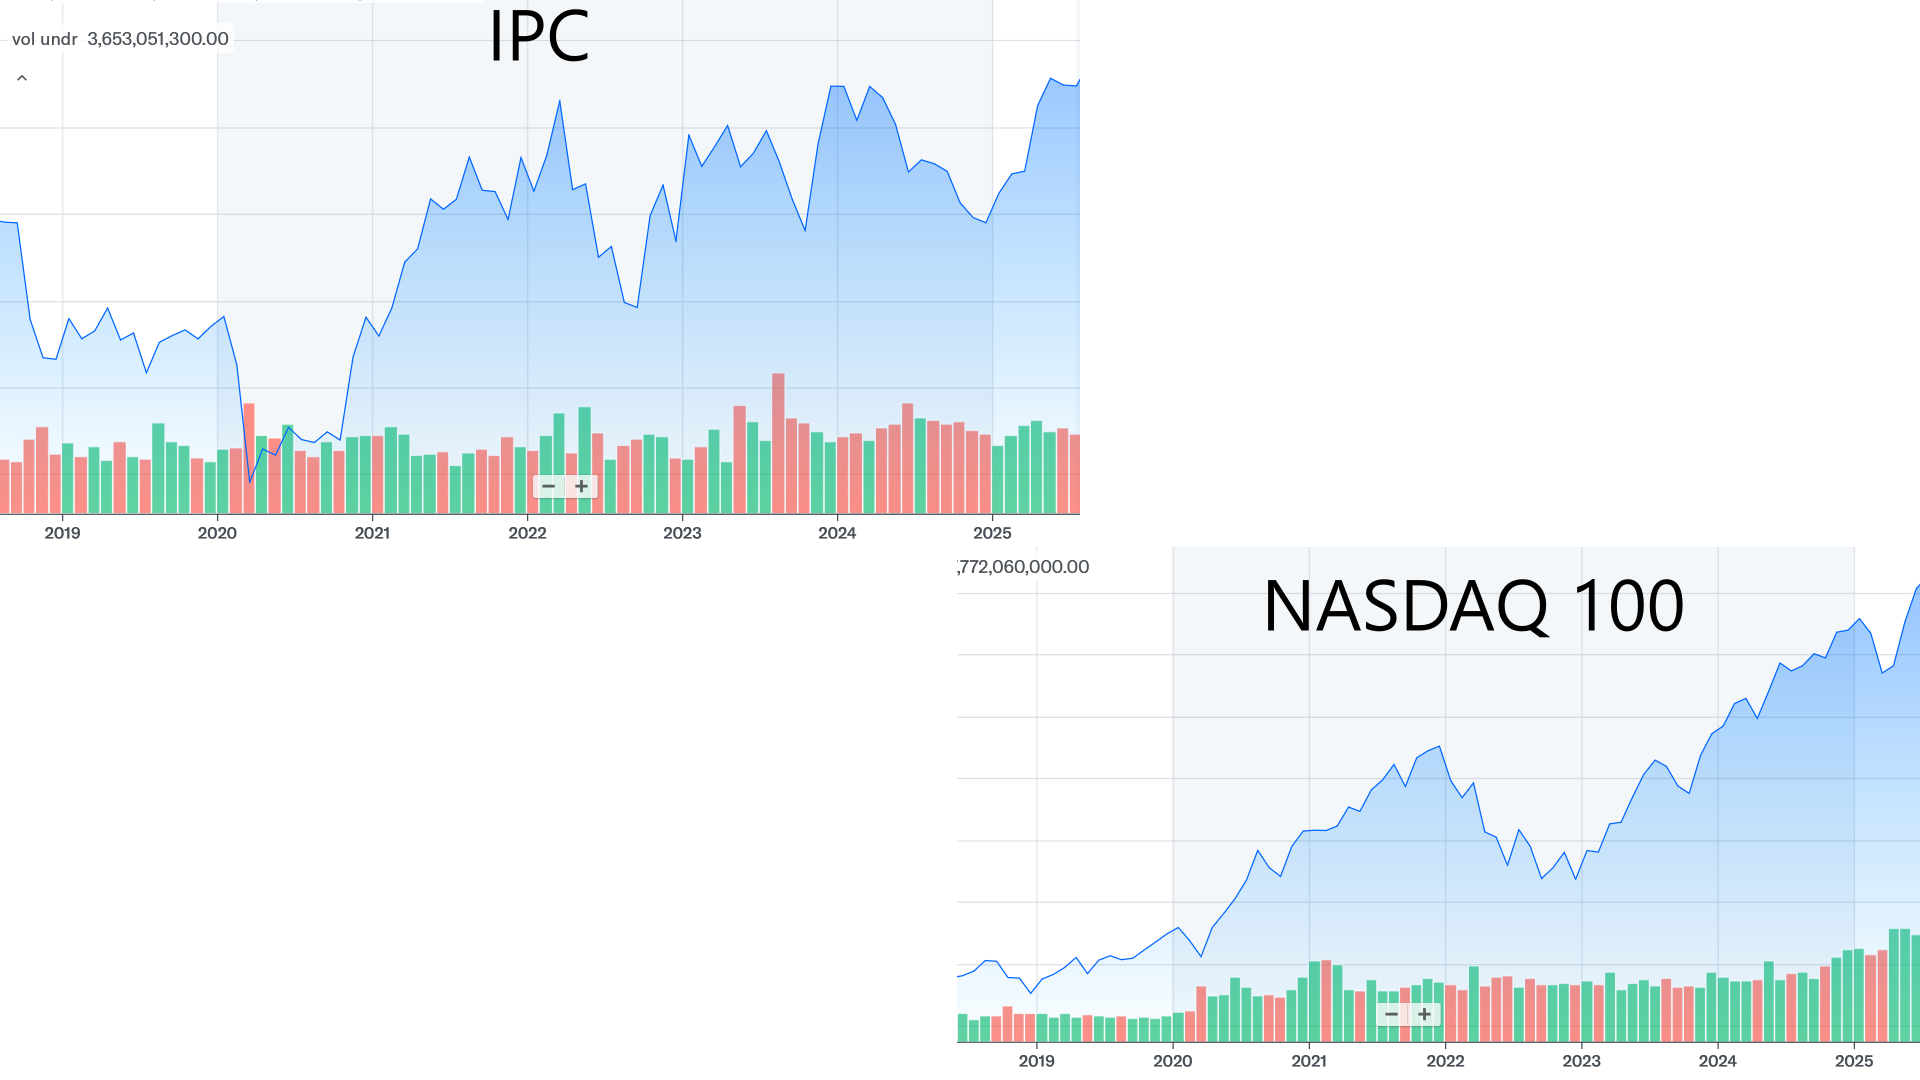
\includegraphics[width=10cm]{indices actuales.png}
    \caption{Valores históricos del IPCy NASDAQ100 (octubre 2018 a julio 2025), junto con volumen mensual. Recuperado de es.finance.yahoo.com}
    \end{figure}
\end{frame}

\begin{frame}{Conceptos previos}
    \begin{block}{\textit{quantitative portfolio managment}}
        Uso de herramientas de la matemática para optimizar la gestión de activos. Radica en dos problemas; uno de clasificación y otro de optimización. 
    \end{block}
    \begin{block}{multilateral insurance}
        Diversificación de un portafolio donde se realizan varias agrupaciones de los activos acorde a una correlación fuerte.
        Koumou (2020)\footnote{Koumou, G. B.(2020) \emph{Diversification and portfolio theory: a review}. Swiss Society for Financial Market Research.}.
    \end{block}
\end{frame}

\begin{frame}{Conceptos previos: \textit{clustering}}
   \begin{block}{Partitioning around medoids}
        Algoritmo para \textit{clustering} similar a \textit{k-means}, pero sin usar medias o distancias euclidianas para 
        asociar a los elementos a un centroide. En su lugar, utiliza cualquier métrica que indique alguna semejanza
        \footnote{Botyarov, M., Miller, E. (2022). \emph{Partitioning around medoids as a systemic approach to 
        generative design solution space reduction.} Elsevier.}
   \end{block}
\end{frame}

\begin{frame}{Conceptos previos: Estrategias}
        \begin{block}{\textit{Risk parity asset allocation}}
        Conjunto de estrategias donde a las acciones se les asignan "pesos", acorde a su volatilidad para repartir el riesgo de manera equitativa.
        \end{block}
         \begin{examples}
        \textit{Equally weighted\footnote{ Chow, T., Hsu, J., Kalesnik, V., Little, B. (2011).},} por capitalización de mercado,
         por volatilidad y \textit{risk parity asset allocation}.
        \footnote{ Chow, T., Hsu, J., Kalesnik, V., Little, B.(2011). \emph{A Survey of Alternative Equity Index Strategies}. Financial Analysts Journal.}
    \end{examples}
\end{frame}

\begin{frame}{Conceptos previos: Discusión}
\begin{itemize}
    \item La diversificacipón no siempre ofrece un enfoque óptimo y tampoco tiene po qué reflejar la realidad del mercado,
     aunque puedan intepretarlo apropiadamente. Además el éxito de un modelo no debe de ser el único criterio para trasponerlo
      en el mundo real, acorde a Choueifaty y Coignard (2008) \footnote{Choueifaty, Y., Coignard, Y. (2008). 
      \emph{Toward Maximum Diversification}. The Journal of Portfolio Management.} .
    \item Todo trabajo de índole búrsatil debe tener al menos dos enfoques, ya que no hay una sola medición que pueda determinar
     la optimalidad de un modelo. Los trabajos como Carvalho \emph{et al.} (2012) \footnote{  Carvalho R. L., Lu, X., Moulin, P.
      (2012).\emph{Demystifying Equity Risk-Based Strategies: A Simple Alpha plus Beta Description}. The Journal of Portfolio Management.},
       enfatizan la importancia de tener más de un enfoque, pero que tampoco es necesario abordar todas las mediciones y estrategias.
    \end{itemize}
\end{frame}

\begin{frame}{Conceptos previos: limitantes de la \textit{modern portfolio theory} de Markowitz}
    \begin{itemize}
        \item Posee datos estáticos y tiende a ser mejor en análisis histórico.
        \item Asume que los retornos se distribuyen de manera normal.
        \item Es bueno para reducir el riesgo no-sistémico bajo la hipótesis de diversidad. Pero es suceptible al riesgo sistémico.
        \item No considera factores macro o estructurales.
    \end{itemize}
\end{frame}

\section{Descripción del problema}
\begin{frame}{Descripción del problema: S\&P/BMV IPC}
    El índice que se busca replicar es el índice de precios y cotizaciones de la bolsa mexicana de valores
    (S\&P/BMV IPC)\footnote{S\&P Dow Jones Indices. (febrero 2025 \emph{S\&P/BMV Indices:
    Metodología})}. \\
    De mayor a menor proporción, el índice representa los sectores:
    \begin{enumerate}
        \item telecomunicaciones
        \item consumo frecuente
        \item materiales
        \item servicios financieros
        \item industrial
        \item servicio y bienes de consumo no básicos
        \item salud
    \end{enumerate}
\end{frame}

\begin{frame}{Descricpión del problema: S\&P/BMV IPC}
    \scriptsize % Puedes cambiar a \scriptsize si necesitas más espacio

    \begin{tabularx}{\textwidth}{>{\raggedright\arraybackslash}X >{\raggedright\arraybackslash}X}
    \toprule
    \textbf{Empresas que conforman el IPC\footnote{S\&P Dow Jones Indices. (31 marzo 2025). S\&P BMV IPC: \emph{Constituents Export}. {[}Base de datos{]}.}} \\
    \midrule
    Alfa S.A. A & Grupo Bimbo S.A.B. \\
    Alsea S.A. & Grupo Carso S.A.B. de C.V. \\
    América Móvil S.A.B. de C.V. B & Grupo Cementos de Chihuahua S.A.B. de C.V. \\
    Arca Continental S.A.B. de C.V. & Grupo Comercial Chedraui S.A. de C.V. \\
    Banco del Bajío S.A. & Grupo Financiero Banorte O. \\
    Becle S.A. De C.V. & Grupo Financiero Inbursa O \\
    Bolsa Mexicana de Valores S.A. de C.V. & Grupo México S.A.B. de C.V. B \\
    Cemex S.A. CPO & Grupo Televisa S.A.B. CPO \\
    Coca Cola Femsa S.A.B. de C.V. UBL & Industrias Peñoles \\
    Corporación Inmobiliaria Vesta S.A.B. de C.V. & Kimberly Clark de México S.A.B. de C.V. A \\
    El Puerto de Liverpool S.A.B. de C.V. & La Comer S.A.B. de C.V. UBC \\
    Fomento Económico Mexicano S.A.B. de C.V. & Megacable Holdings S.A.B. de C.V. \\
    Genomma Lab Internacional S.A. de C.V. & Orbia Advance Corporation S.A.B. de C.V. \\
    Gentera S.A.B. de C.V. & Promotora y Operadora de Infraestructura SAB de CV \\
    Gruma S.A.B. B & Qualitas Controladora S.A.B. de C.V. \\
    Grupo Aeroportuario del Centro Norte S.A.B. de C.V. & Regional S.A. de C.V. \\
    Grupo Aeroportuario del Pacifico, S.A.B. de C.V. & Walmart de México S.A.B. de C.V. \\
    Grupo Aeroportuario del Sureste S.A.B. de C.V. B & \\
    \bottomrule
    \end{tabularx}
\end{frame}

\begin{frame}{Descripción del problema}
    \quad Utilizando las librerías \texttt{yfinance} e \texttt{invest-corepy} en Visual Basic 1.99.3 con Python 3.12.7 
    integrado en el paquete de anaconda de versión 2.6.5, se obtuvieron los datos históricos desde Yahoo
    Finance de los precios máximos, mínimos y de cierre, volumennes, además de la cantidad en circulación 
    de las acciones de las 35 empresas durante los períodos 2008 a 2010 y 2015 a 2024.

    \quad Los datos del estado del IPC diario fueron tomados de Banco de México \footnote{Banco de México. 
    (2025). Sistema de Información Económica {[}Base de datos{]}.}. Y todo el programa se realizó en una
    serie de notebooks de Jupyter (v2025.9.1) utilizando el antes mencioado paquete de anaconda.
    Además, las instancias de optimización con Markowitz fueron resueltas con un modelo general construido en Gurobi 12.0.0.
\end{frame}

\begin{frame}{Descripción del problema: Obtención de datos}
    \quad Los portafolios, excepto el del clustering y el \emph{equally weighted} que por su naturaleza
    son fijos, pero el resto van a estarse reajustando cada 6 meses. Lo ideal es tener distintos períodos
    para reajustarse, pero tomamos los 6 meses porque es la misma cantidad de tiempo en la que IPC se
    requilibra, para así tener una consistencia entre nuestro portafolio y el índice.
\end{frame}
\begin{frame}{Descripción del problema: Modelo para \textit{clustering}}
    \begin{block}{Función objetivo para \textit{clustering}}
    \begin{equation}
\max\sum_{i = 1}^{n}{\sum_{j = 1}^{n}{c_{ij}x_{ij}}} \tag{1}
\end{equation}
    \end{block}
        \begin{columns}

    % Columna izquierda - Ecuaciones
    \begin{column}{0.5\textwidth}
        \small
        Sujeto a:
        \begin{equation}
        \sum_{j = 1}^{n} y_{j} = k \tag{1.2}
        \end{equation}
        \begin{equation}
        \sum_{j = 1}^{n} x_{ij} = 1\quad \forall i \tag{1.3}
        \end{equation}
        \begin{equation}
        x_{ij} \leq y_{j} \quad \forall i,j \tag{1.4}
        \end{equation}
        \begin{equation}
        x_{ij}, y_{j} \in \{0,1\} \tag{1.5}
        \end{equation}
    \end{column}

    % Columna derecha - Tabla
    \begin{column}{0.5\textwidth}
        \small
        \begin{tabularx}{\textwidth}{@{}lX@{}}
        \toprule
        $c_{ij}$ & Similitud entre activo $i$ y $j$. Correlación entre ambos activos (valores entre -1 y 1). \\
        \midrule
        $x_{ij}$ & 1 si el activo $j$ tiene alta correlación positiva con el activo $i$, 0 de lo contrario. \\
        \midrule
        $y_j$ & 1 si el activo $j$ está en el portafolio, 0 en caso contrario. \\
        \midrule
        $k$ & Cantidad de centroides o activos representativos (menor que el total de activos). \\
        \bottomrule
        \end{tabularx}
       % \captionof*{table}{Descripción de las variables del modelo de \textit{k-medoids}.}
    \end{column}
\end{columns}
\end{frame}

\begin{frame}{\textit{Benchmarks: Equally weighted}}
    \begin{block}{Función de asignación de "pesos" (EW)}
        \begin{equation}
            w_{i} = \frac{1}{n} \tag{2}   
        \end{equation}
    \end{block}
    \vspace{0.5cm}
    \small % Reduce el tamaño del texto si es necesario

    \begin{tabularx}{\textwidth}{@{}lX@{}}
        \toprule
        $w_{i}$ & Peso del activo \emph{i}, es decir, su importancia y cuánto debe invertirse en comparación con el resto. \\
        \midrule
        $n$ & Total de activos. \\
        \bottomrule
    \end{tabularx}
\end{frame}

\begin{frame}{\textit{Benchmarks: }Capitalización de mercado}
        \begin{block}{Función de asignación de "pesos" (MC)}
        \begin{equation}
            w_{i} = \frac{M_{i}}{\sum_{j}^{n}M_{j}}   \tag{3}
        \end{equation}
    \end{block}
    \begin{columns}

    % Columna izquierda - Ecuaciones
    \begin{column}{0.5\textwidth}
        \small
        Sujeto a:
        \begin{equation}
        M_{i} = x_{i}p_{i} \tag{4.1}   
        \end{equation}
    \end{column}

    % Columna derecha - Tabla
    \begin{column}{0.5\textwidth}
        \small
\begin{tabularx}{\textwidth}{@{}lX@{}}
    \toprule
    $M_{i}$ & Capitalización del mercado de la compañía \emph{i}. Puede entenderse como una métrica para evaluar la viabilidad de invertir en una compañía. Al dividir esta medida entre la suma total de capitalizaciones, se obtiene la proporción con la que se debería invertir en cada compañía. \\
    \midrule
    $x_{i}$ & Cantidad de acciones circulando en el mercado de la compañía \emph{i}. \\
    \midrule
    $p_{i}$ & Precio actual de las acciones de la compañía \emph{i}. \\
    \bottomrule
    \end{tabularx}
        % \captionof*{table}{Descripción de las variables del modelo de \textit{k-medoids}.}
        \end{column}
    \end{columns}
\end{frame}

\begin{frame}{\textit{Benchmarks: }Volatilidad}
    \begin{block}{Función de asignación de "pesos" (Vol)}
        \begin{equation}
            w_{i} = \frac{\frac{1}{\sigma_{i}}}{\sum_{j}^{n}\frac{1}{\sigma_{j}}}   \tag{5}
        \end{equation}
    \end{block}
    \begin{tabularx}{\textwidth}{@{}
        >{\raggedright\arraybackslash}p{0.15\textwidth}
        >{\raggedright\arraybackslash}X@{}}
        \toprule
        $\sigma_i$ & Volatilidad del activo \emph{i}. La desviación estándar de su precio. \\
        \bottomrule
    \end{tabularx}
\end{frame}

\begin{frame}{Asignación de pesos representativos}
    \begin{block}{Modelo de asignación de pesos de acciones representativas}
        \begin{equation}
            x_{jl} = \frac{\sum_{i \in C_{l}}^{}w_{i}}{\sum_{I = 1}^{n}w_{i}},\ \ l = 1,\ldots,\ k  \tag{6} 
        \end{equation}
    \end{block}
    \begin{tabularx}{\textwidth}{@{}
        >{\raggedright\arraybackslash}p{0.4\textwidth}
        >{\raggedright\arraybackslash}X@{}}
        \toprule
        $w_{i}$ & Peso del activo $i$ dentro de un determinado portafolio \\
        \midrule
        $C_{l}$ & Clúster $l$ \\
        \midrule
        \emph{l} & Cantidad de clústeres \\
        \midrule
        $x_{jl}$ & Peso de la acción representativa $j$ en el clúster $l$ \\
        \bottomrule
    \end{tabularx}
%Tener en consideraciòn el citar las tablas
%\vspace{0.5em}
%\small
%\textbf{Fuente:} Elaboración propia. Descripción de variables para asignar pesos optimizados según los activos representativos de la clusterización y la capitalización de mercado.
\end{frame}
\begin{frame}{Optimización de pesos}
    \begin{block}{Función objetivo para optimización en construcción de portafolios multidimensional}
        \begin{equation}
        \min{\left( X - X_{B} \right)^{T}M(X - X_{B}}) \tag{7}  
        \end{equation}
    \end{block}
    \begin{columns}
        \begin{column}{0.5\textwidth}
            \small
            Sujeto a:
            \begin{equation}
            1^{T}X = 1 \tag{7.2}    
            \end{equation}
            \begin{equation}
            X \geq 0 \tag{7.3}    
            \end{equation}
            \begin{equation}
            \left| w_{i} - w_{b,i} \right| < turnover \tag{7.4}
            \end{equation}
            \begin{equation}
            \sum_{i = 1}^{n}{\left| w_{i} - w_{b,i} \right| \leq t}   \tag{7.5}
            \end{equation}
        \end{column}
        \begin{column}{0.5\textwidth}
            \small
            \begin{tabularx}{\textwidth}{@{}
                >{\raggedright\arraybackslash}p{0.18\textwidth}
                >{\raggedright\arraybackslash}X@{}}
                \toprule
                \emph{X} & Nuestra variable, el portafolio con pesos optimizados \\
                \midrule
                $X_b$ & Vector con los pesos de los activos representativos dado un cierto \textit{benchmark} y \textit{clustering} \\
                \midrule
                \emph{M} & Matriz de covarianza de los rendimientos de los activos representativos\\
                \bottomrule
            \end{tabularx}

            \vspace{0.5em}
            \small
            \textbf{Fuente:} Choueifaty y Coignard (2008).
        \end{column}    
    \end{columns}
\end{frame}

\begin{frame}{Medición del error}
    \begin{block}{Rendimiento en un período \textit{i} de longitud 1}
        \begin{equation}
            rendimiento_{i} = \frac{v_{i}(t)-v_{i}(t-1)}{v_{i}(t-1)} \tag{8}   
        \end{equation}
    \end{block}
    \vspace{0.5cm}
    \begin{block}{Error de seguimiento}
        \begin{equation}
            TE = desvstd(rendimiento_{p,t}-rendimiento_{idx,t})  \tag{9}   
        \end{equation}
    \end{block}
    \vspace{0.5cm}    
    \small % Reduce el tamaño del texto si es necesario
    \begin{tabularx}{\textwidth}{@{}lX@{}}
    \toprule
    $v_{i}(t)$ & valor del activo \emph{i} en el período t \\
    \midrule
    $TE$ & \textit{Tracking error}, volatilidad de la diferencia en los retornos \\
    \bottomrule
    \end{tabularx}
\end{frame}

\section{Resultados}
\begin{frame}{Asignación de activos — 2 Clústeres (1/2)}
    \small
    \textbf{Empresas representativas para 2 clústeres}

    \vspace{0.8em}

    \begin{tabularx}{\textwidth}{@{}X X@{}}
    \toprule
    \textbf{Clúster 1} & \textbf{Clúster 2} \\
    \midrule
    Grupo Financiero Banorte O & Grupo Televisa S.A.B. CPO\\  
    Grupo Bimbo S.A.B. & Alfa S.A. A. \\
    Alsea S.A. & Banco del Bajío S.A. \\
    Cemex S.A. C.P.O. & Bolsa Mexicana de Valores S.A. de C.V. \\
    Arca Continental S.A.B. de C.V. & Industrias Peñoles \\
    Banco del Bajío S.A. & Megacable Holdings S.A.B. de C.V.\\
    Grupo Carso S.A.B. de C.V. & Orbia Advance Corporation S.A.B. de C.V.  \\
    Coca Cola Femsa S.A.B. de C.V. UBL & \\
    Corporación Inmobiliaria Vesta S.A.B. de C.V. & \\
    El Puerto de Liverpool S.A.B. de C.V. & \\
    Fomento Económico Mexicano S.A.B. de C.V. & \\
    Grupo Financiero Inbursa O. & \\
    América Móvil S.A.B. de C.V. B &  \\
    Becle S.A. De C.V. & \\
    \bottomrule
    \end{tabularx}
\end{frame}

\begin{frame}{Asignación de activos — 2 Clústeres (2/2)}
    \small

    \begin{tabularx}{\textwidth}{@{}X X@{}}
        \toprule
        \textbf{Clúster 1} & \textbf{Clúster 2} \\
        \midrule
        Qualitas Controladora S.A.B. de C.V. & \\
        Genomma Lab Internacional S.A. de C.V. & \\
        Gentera S.A.B. de C.V. & \\
        Gruma S.A.B. B & \\
        Grupo Aeroportuario del Centro Norte S.A.B. de C.V. & \\
        Grupo Aeroportuario del Sureste S.A.B. de C.V. & \\
        Grupo Cementos de Chihuahua S.A.B. de C.V. & \\
        Grupo Comercial Chedraui S.A. de C.V. & \\
        Grupo México S.A.B. de C.V. B & \\
        Kimberly Clark de México S.A.B. de C.V. A & \\
        La Comer S.A.B. de C.V. UBC & \\
        Regional S.A. de C.V. &  \\
        Walmart de México S.A.B. de C.V. & \\
        \bottomrule
    \end{tabularx}
\end{frame}

% ===== Tabla 2: 4 Clústeres =====
\begin{frame}{Asignación de activos — 4 Clústeres (1/2)}
    \small
    \textbf{Empresas representativas para 4 clústeres}

    \vspace{0.8em}

    \begin{tabularx}{\textwidth}{@{}X X X X@{}}
        \toprule
        \textbf{C1} & \textbf{C2} & \textbf{C3} & \textbf{C4} \\
        \midrule
        Bolsa Mexicana de Valores & Genomma Lab Internacional & Grupo Financiero Banorte & Grupo Televisa \\
        Becle &  & Grupo Bimbo & Megacable Holdings \\
        Industrias Peñoles &  & Fomento Económico Mexicano  & Orbia Advance Corporation \\
        La Comer & & Alsea & \\
        & & América Móvil & \\
        & & Arca Continental & \\
        & & Banco del Bajío & \\
        & & Coca Cola Femsa & \\
        & & Corporación Inmobiliaria Vesta & \\
        & & El Puerto de Liverpool & \\
        & & Cemex & \\
        \bottomrule
    \end{tabularx}

\end{frame}

\begin{frame}{Asignación de activos — 4 Clústeres (2/2)}
    \small

    \begin{tabularx}{\textwidth}{@{}X X X X@{}}
        \toprule
        \textbf{C1} & \textbf{C2} & \textbf{C3} & \textbf{C4} \\
        \midrule
        & & Gentera & \\
        & & Gruma & \\
        & & Grupo Aeroportuario Centro Norte &  \\
        & & Grupo Aeroportuario Sureste & \\
        & & Grupo Comercial Chedraui &   \\
        & & Grupo Financiero Inbursa & \\
        & & Grupo México &  \\
        & & Kimberly Clark de México &  \\
        & & Qualitas Controladora &  \\
        & & Regional & \\
        & & Walmart de México & \\
        \bottomrule
    \end{tabularx}
\end{frame}

% ===== Tabla 3: 8 Clústeres =====
\begin{frame}{Asignación de activos — 8 Clústeres (1/2)}
    \small
    \textbf{Empresas representativas para 8 clústeres}
    \vspace{0.8em}
    \begin{tabularx}{\textwidth}{@{}X X X X X X X X@{}}
        \toprule
        \textbf{C1} & \textbf{C2} & \textbf{C3} & \textbf{C4} & \textbf{C5} & \textbf{C6} & \textbf{C7} & \textbf{C8} \\
        \midrule
        Alfa  & América Móvil & Arca Continental & Bolsa Mexicana  & Genomma Lab & Grupo Carso & Grupo México & Televisa \\
        & & Bimbo & Becle & & Alsea & Cemex & Megacable \\
        & & Bajío & Peñoles & & Vesta  & Cementos Ch & \\
        & & Femsa & Qualitas & & Fomento & La Comer & \\
        & & Liverpool & & & Gentera & & \\
        & & Banorte & & & Gruma & & \\
        \bottomrule
    \end{tabularx}
    \vspace{0.5em}
\end{frame}

\begin{frame}{Asignación de activos — 8 Clústeres (2/2)}
    \small
    \begin{tabularx}{\textwidth}{@{}X X X X X X X X@{}}
        \toprule
        \textbf{C1} & \textbf{C2} & \textbf{C3} & \textbf{C4} & \textbf{C5} & \textbf{C6} & \textbf{C7} & \textbf{C8} \\
        \midrule
        & & Inbursa & & & Aeroportuario Norte & & \\
        & & Chedrahui & & & Aeroportuario Sureste & & \\
        & & Regional & & & & Kimberly Clark & \\
        & & Walmart & & & & & \\
        \bottomrule
    \end{tabularx}
\end{frame}

\begin{frame}{Resultados: Error de seguimiento en portafolio \textit{benchmark}}
    \begin{figure}[htp]
    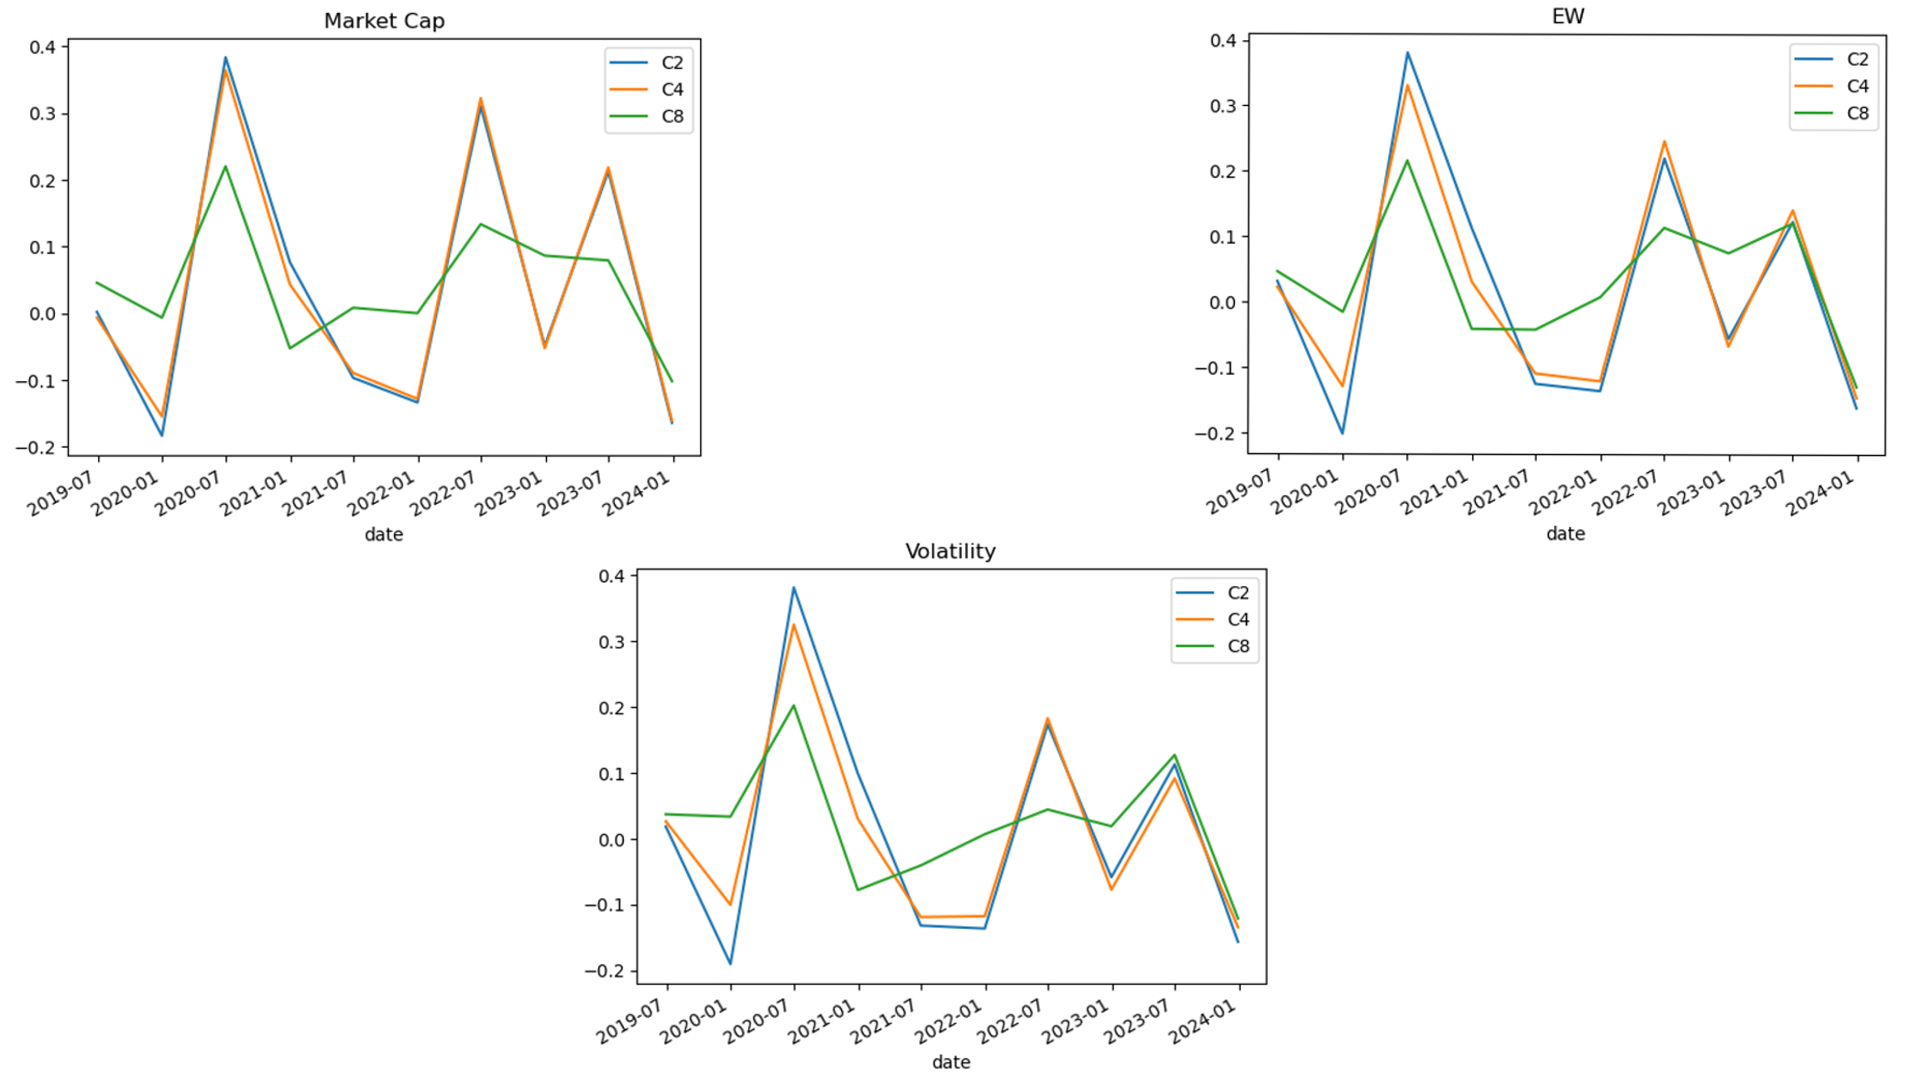
\includegraphics[width=10cm]{sin optimizar por tipo por tiempo.png}
    \caption{Error de seguimiento de portafolios con pesos del \textit{benchmark} con respecto
    al IPC S\&P/BMV según tipo de \textit{benchmark} y \textit{clustering} con respecto al tiempo}
    \end{figure}
\end{frame}

\begin{frame}{Resultados: Error de seguimiento en portafolio \textit{benchmark}}
    \begin{figure}[htp]
        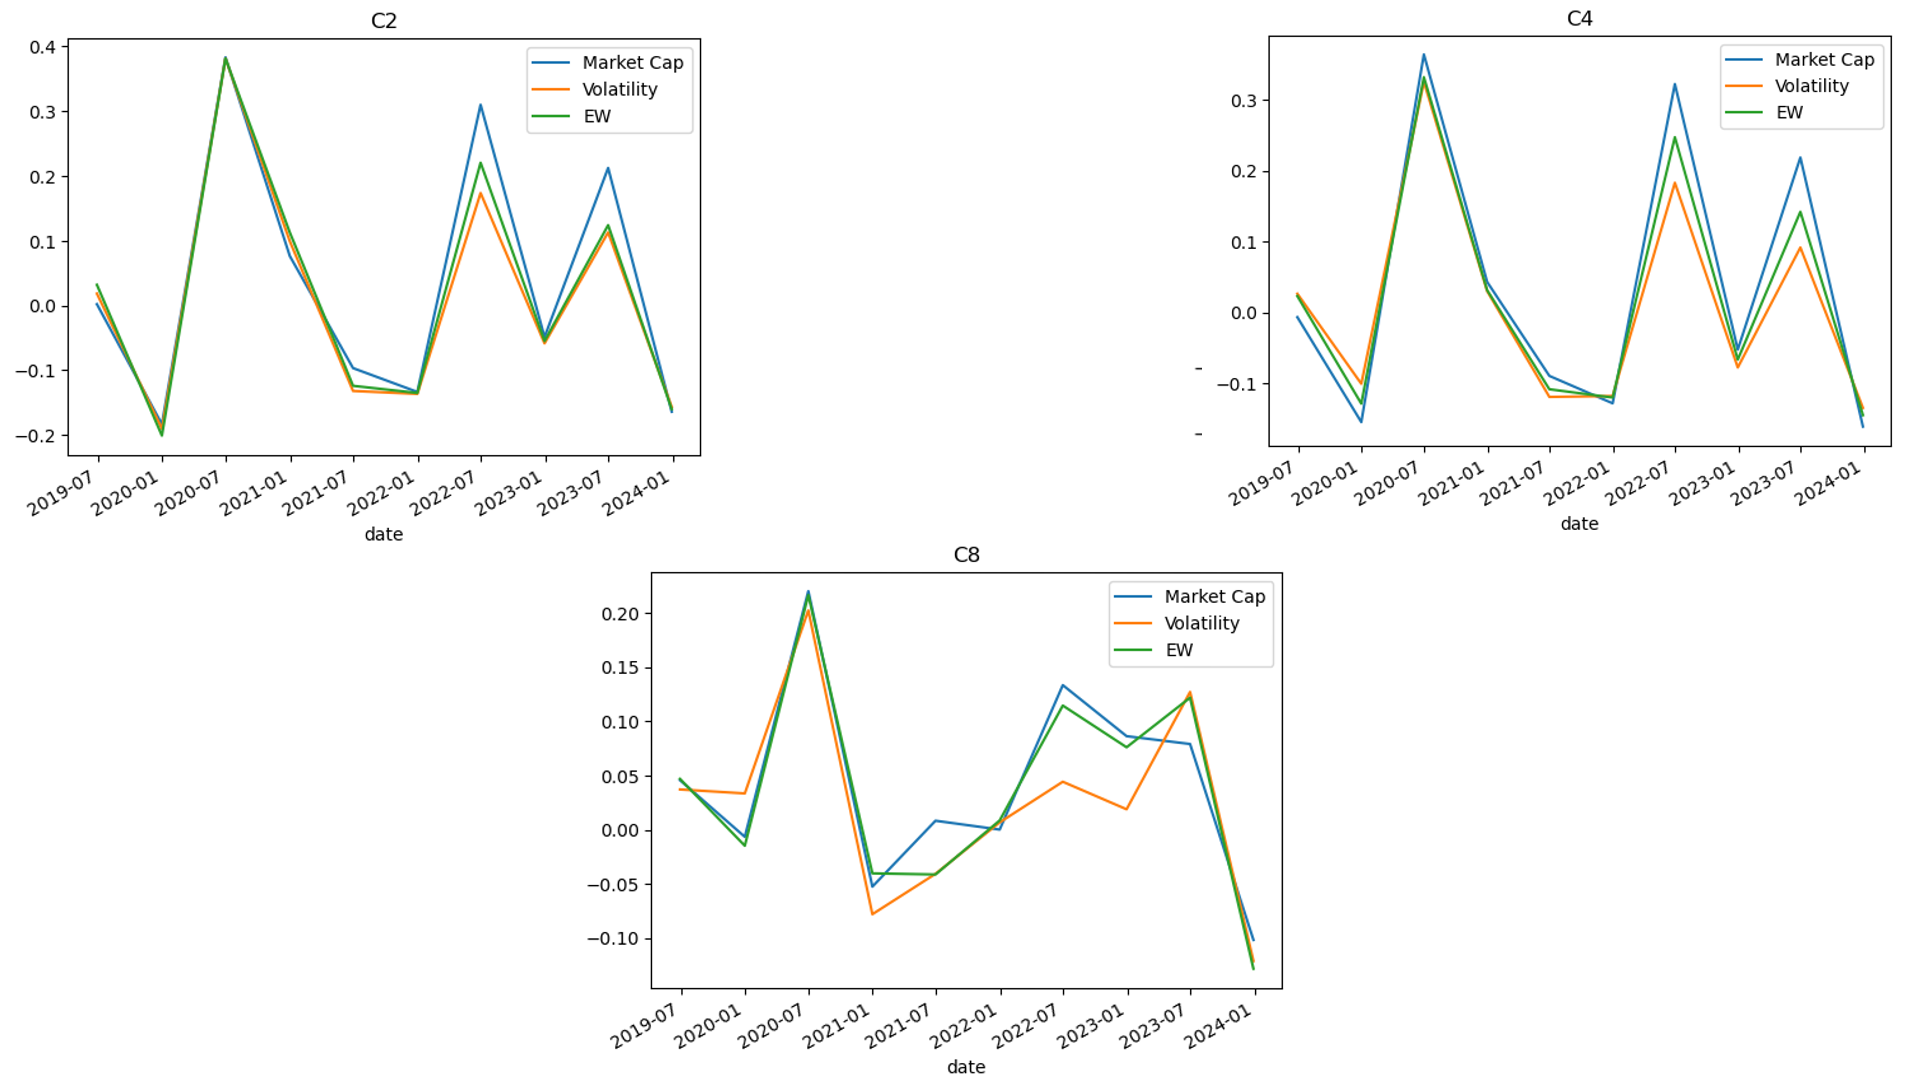
\includegraphics[width=10cm]{sin optimizar por cluster por tiempo.png}
        \caption{Error de seguimiento de portafolios con pesos del \textit{benchmark} con respecto
        al IPC S\&P/BMV según \textit{clustering} y tipo de \textit{benchmark}, con respecto al tiempo}
    \end{figure}
\end{frame}

\begin{frame}{Resultados: Error de seguimiento en portafolio \textit{benchmark}}
    \begin{figure}[htp]
        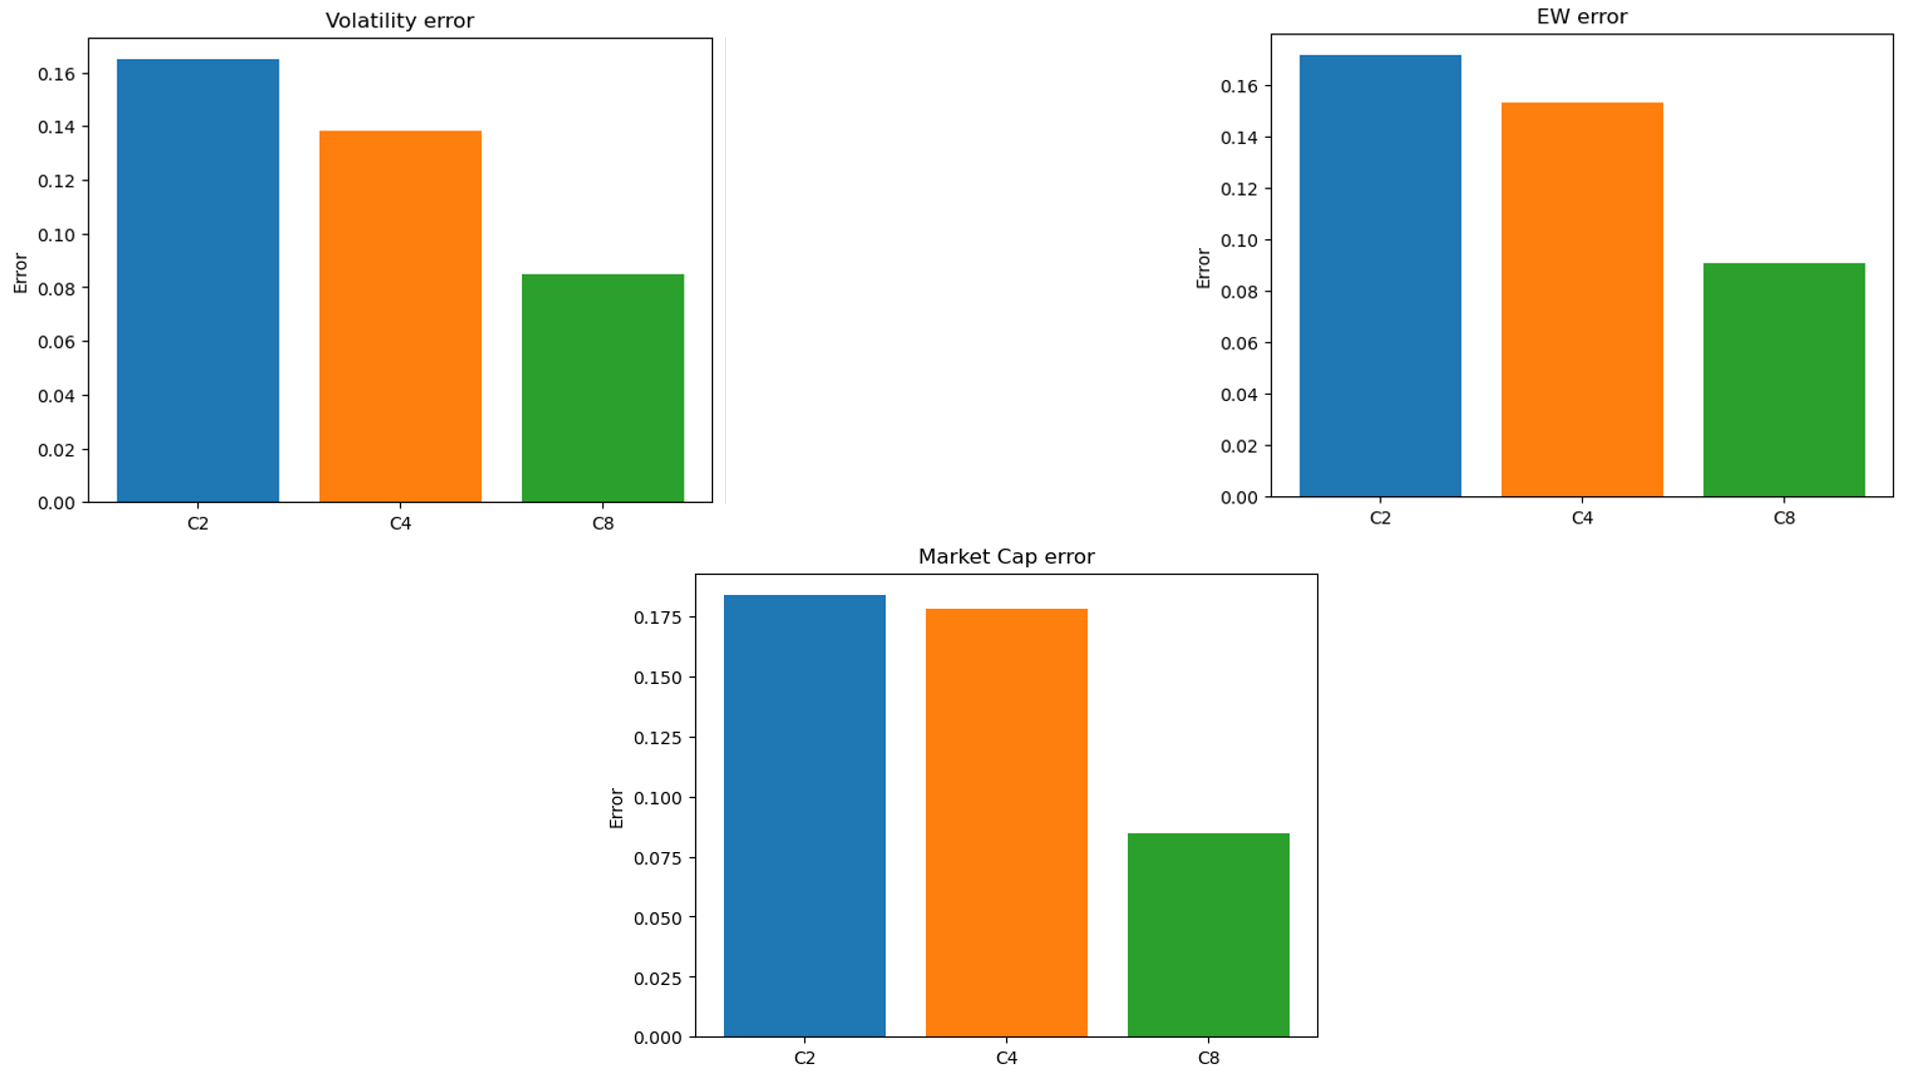
\includegraphics[width=10cm]{sin optimizar total por tipo.png}
        \caption{Error total de seguimiento de portafolios con pesos del \textit{benchmark} con respecto 
        al IPC S\&P/BMV según tipo de \textit{benchmark}.}
    \end{figure}
\end{frame}

\begin{frame}{Resultados: Error de seguimiento en portafolio \textit{benchmark}}
    \begin{figure}[htp]
        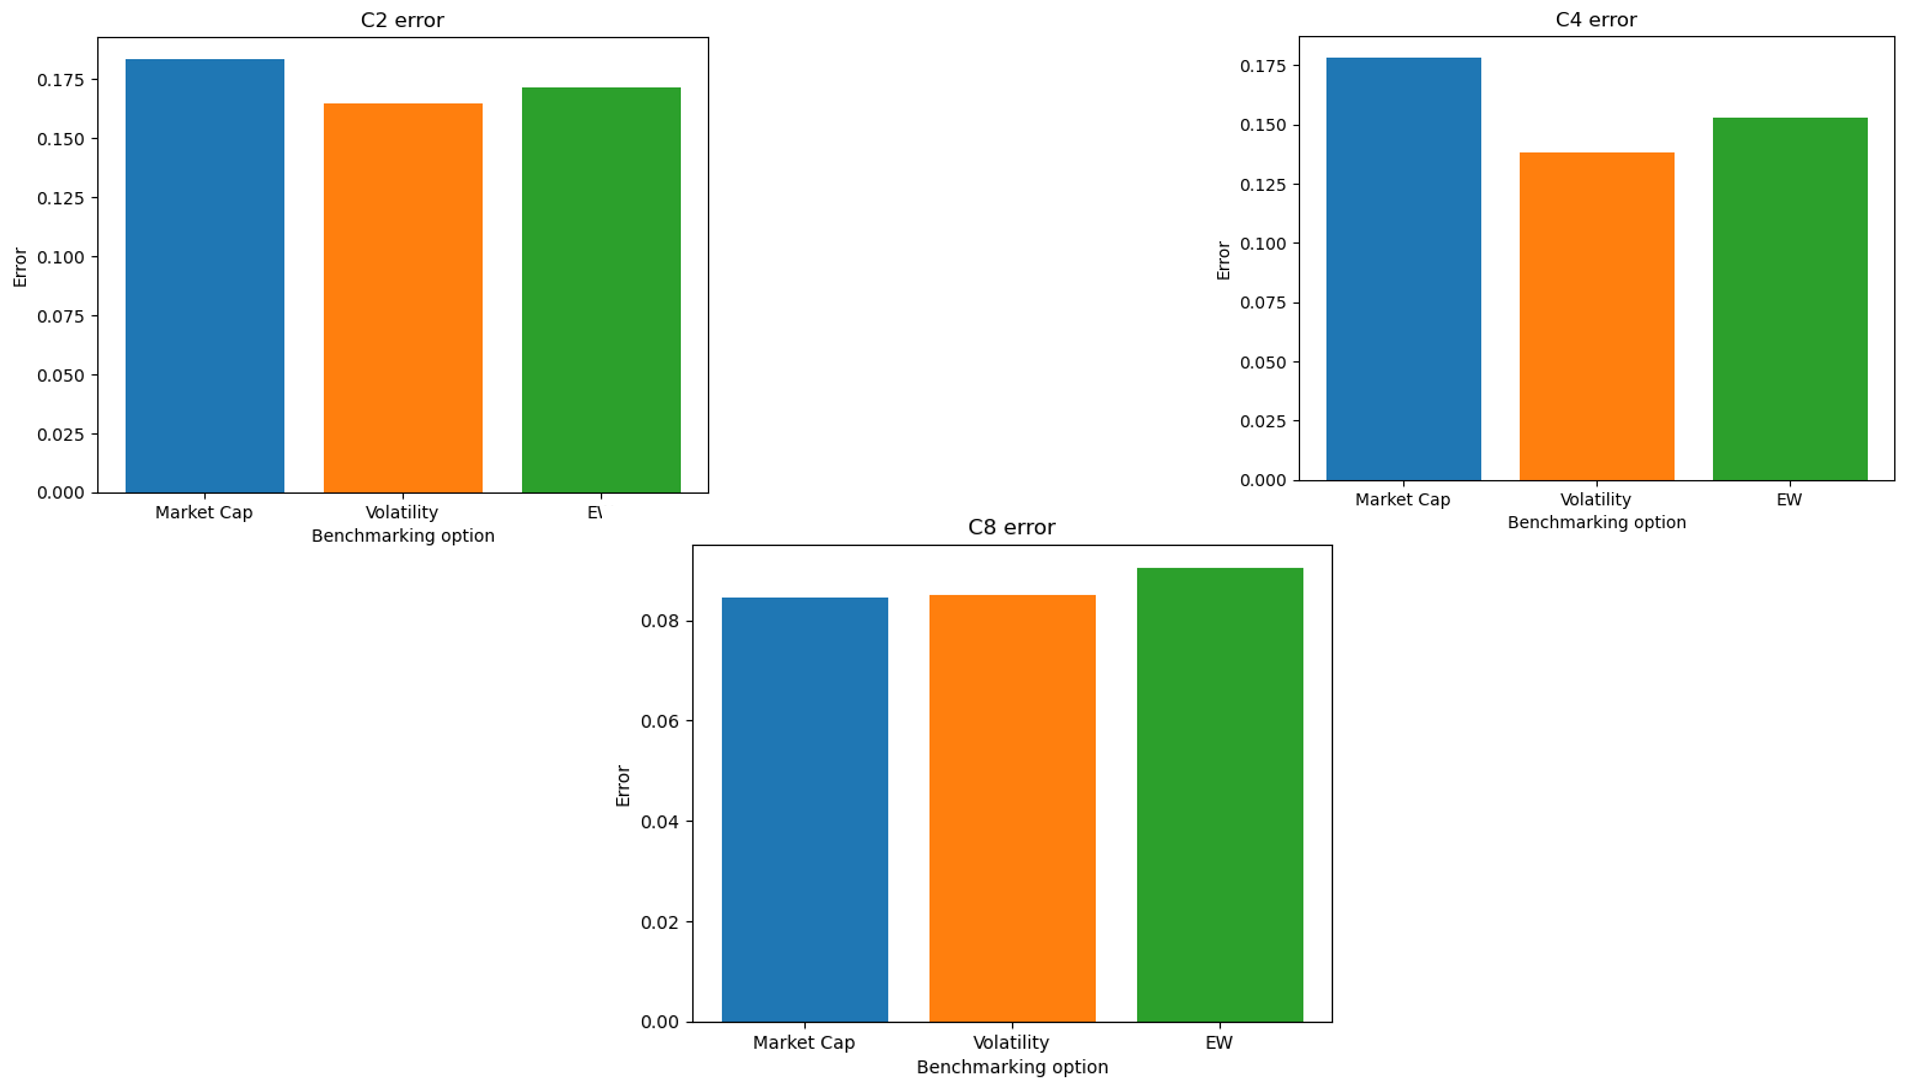
\includegraphics[width=10cm]{sin optimizar total por clusters.png}
        \caption{Error total de seguimiento de portafolios con pesos del \textit{benchmark} con respecto al 
        IPC S\&P/BMV según \textit{clustering}.}
    \end{figure}
\end{frame}

\begin{frame}{Resultados: Error de seguimiento en portafolio \textit{benchmark}}
    \begin{figure}[htp]
        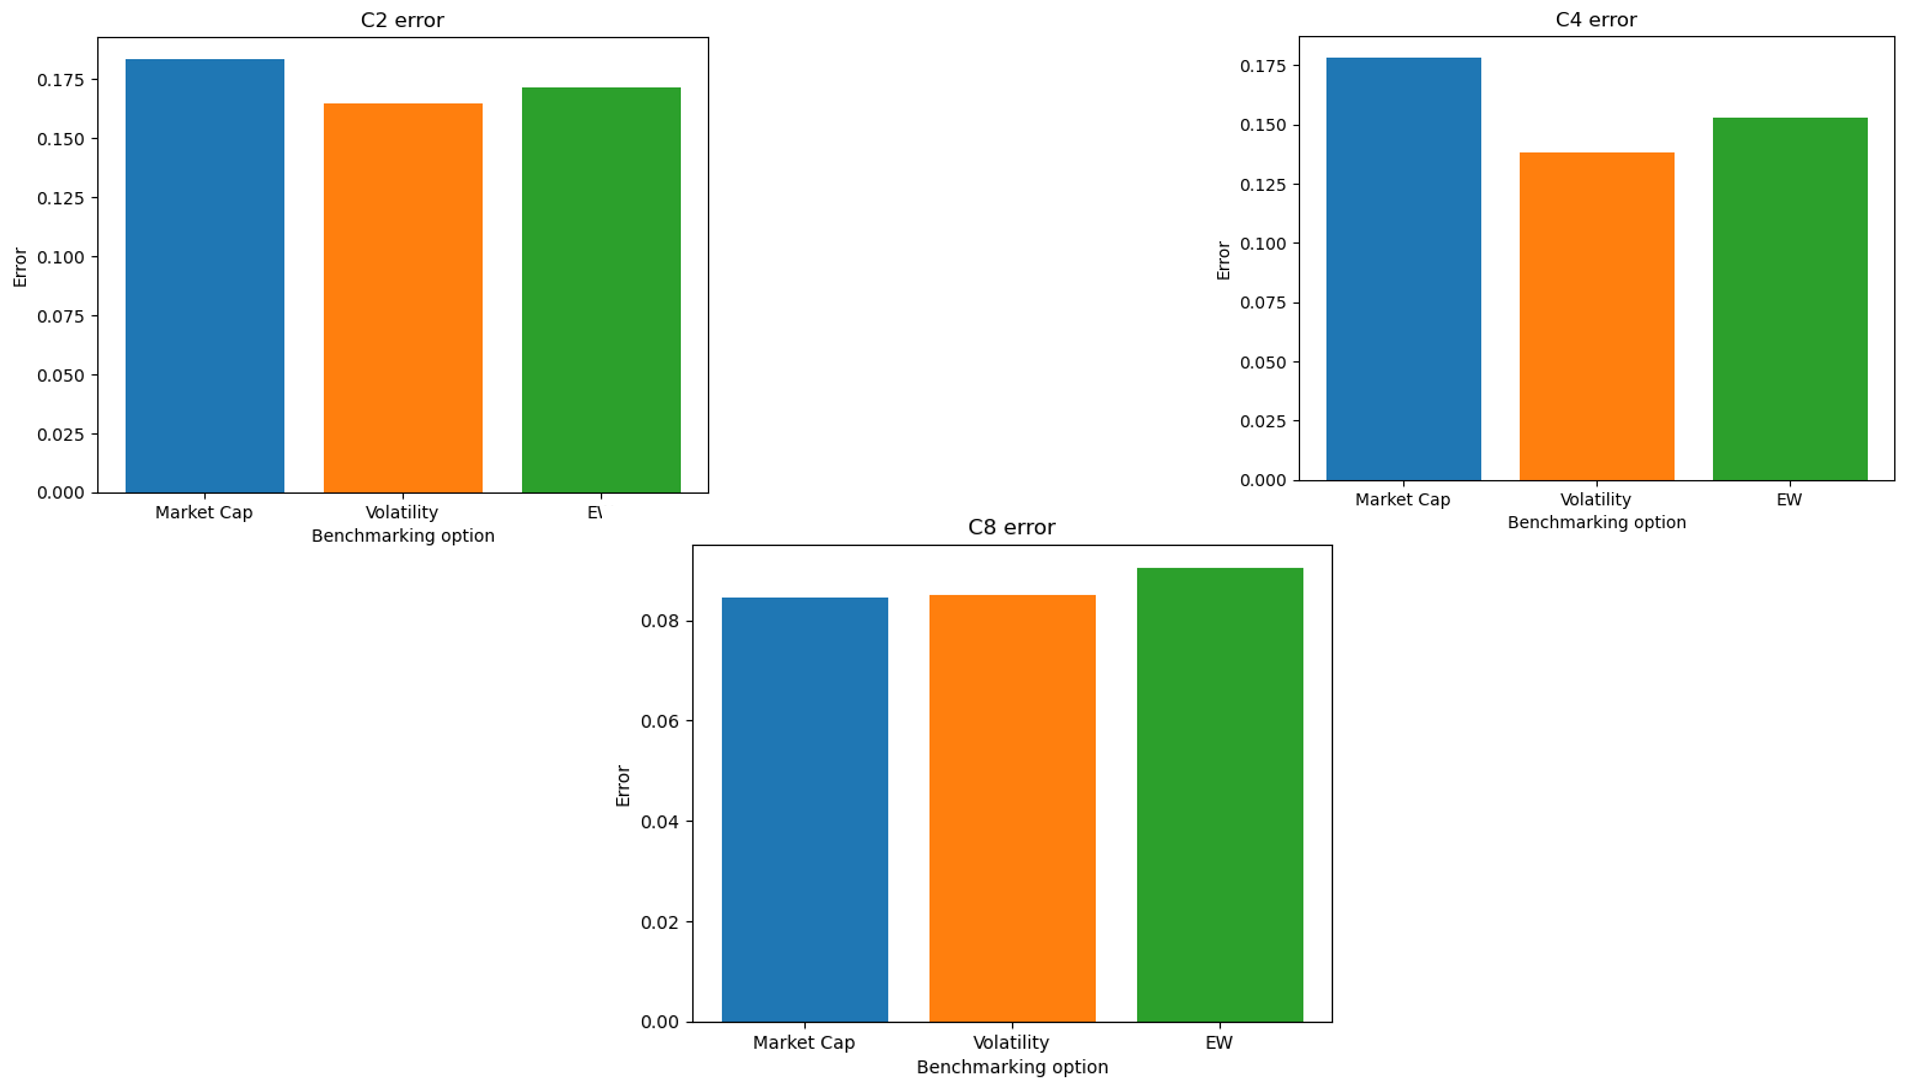
\includegraphics[width=10cm]{sin optimizar total por clusters.png}
        \caption{Error total de seguimiento de portafolios con pesos del \textit{benchmark} con respecto al 
        IPC S\&P/BMV según \textit{clustering}.}
    \end{figure}
\end{frame}

\begin{frame}{Resultados: Error de seguimiento en portafolio optimizado con Markowitz pero no acotado}
    \begin{figure}[htp]
        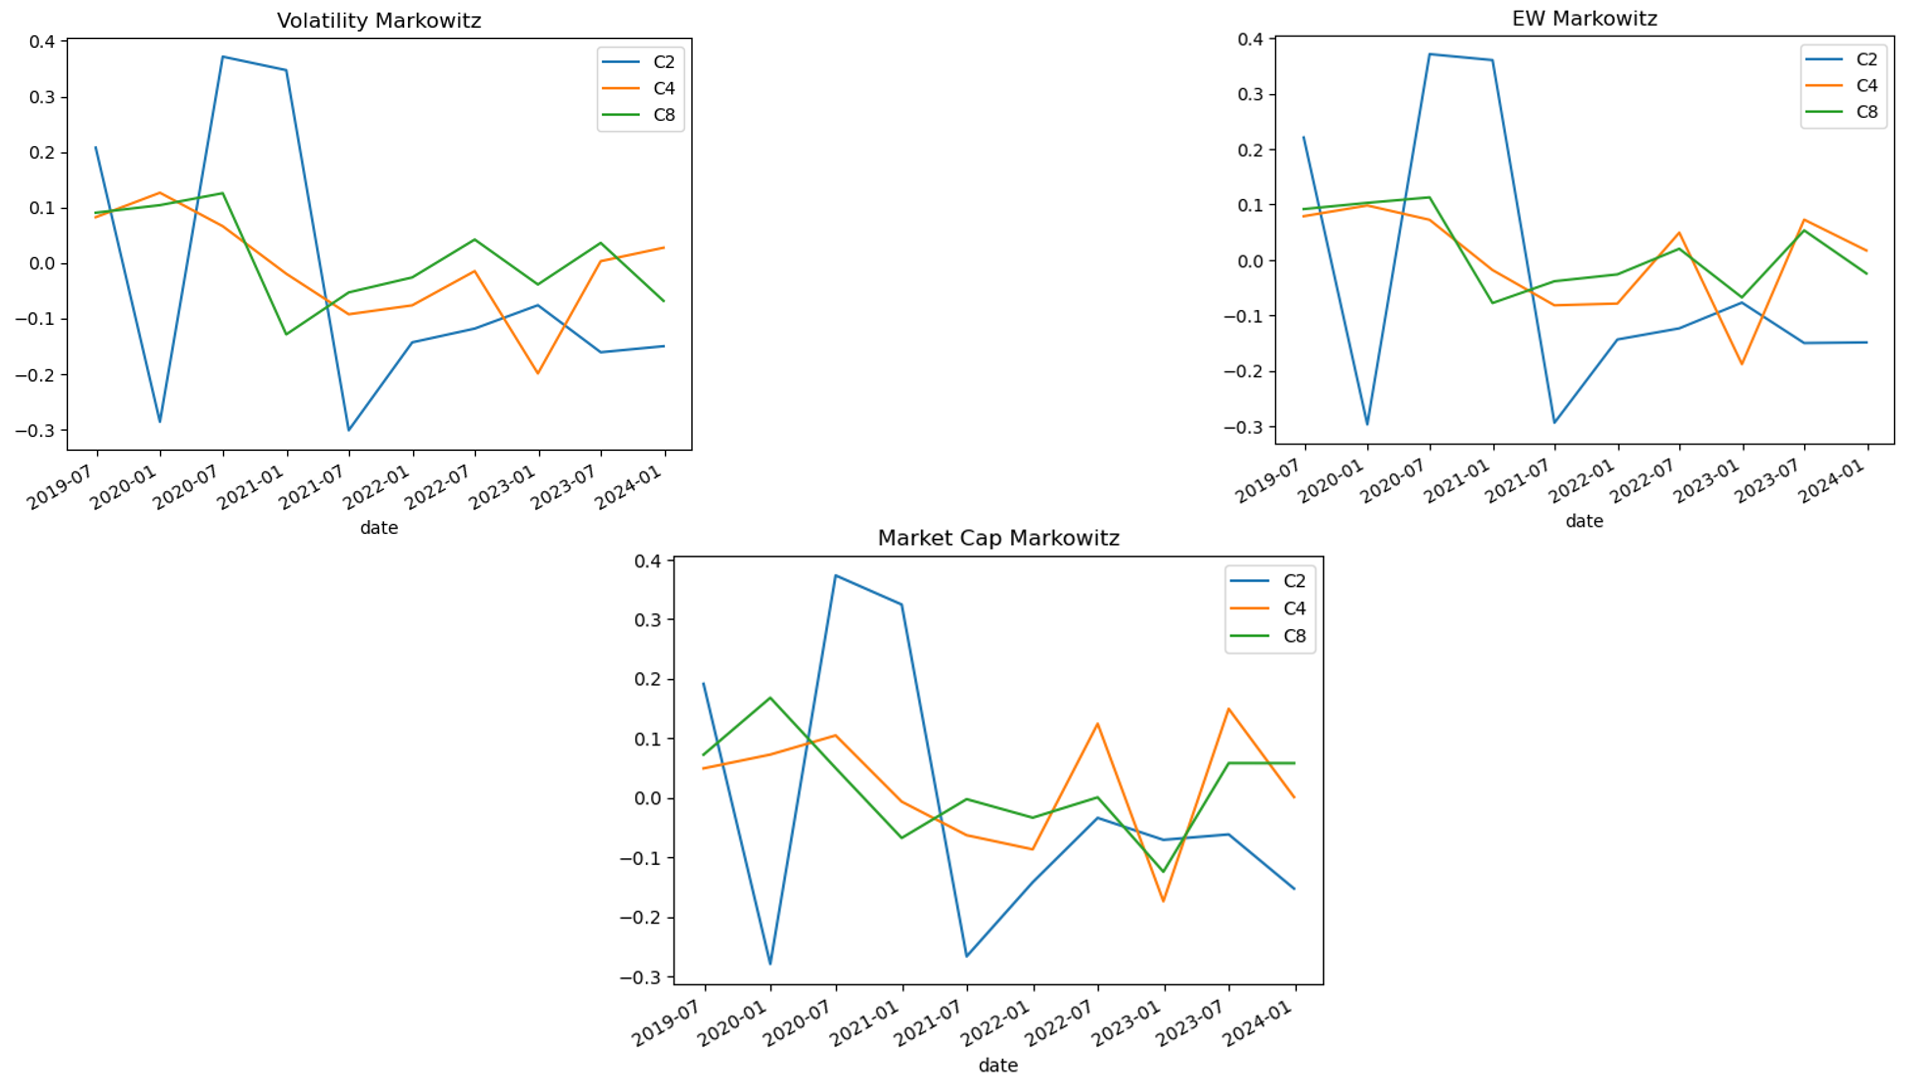
\includegraphics[width=10cm]{optimizado no acotado por tipo por tiempo.png}
        \caption{Error de seguimiento de portafolios con pesos optimizados con Markowitz pero no acotados, 
        con respecto al IPC S\&P/BMV según tipo de \textit{benchmark} y \textit{clustering} con respecto al tiempo}
    \end{figure}
\end{frame}

\begin{frame}{Resultados: Error de seguimiento en portafolio optimizado con Markowitz pero no acotado}
    \begin{figure}[htp]
        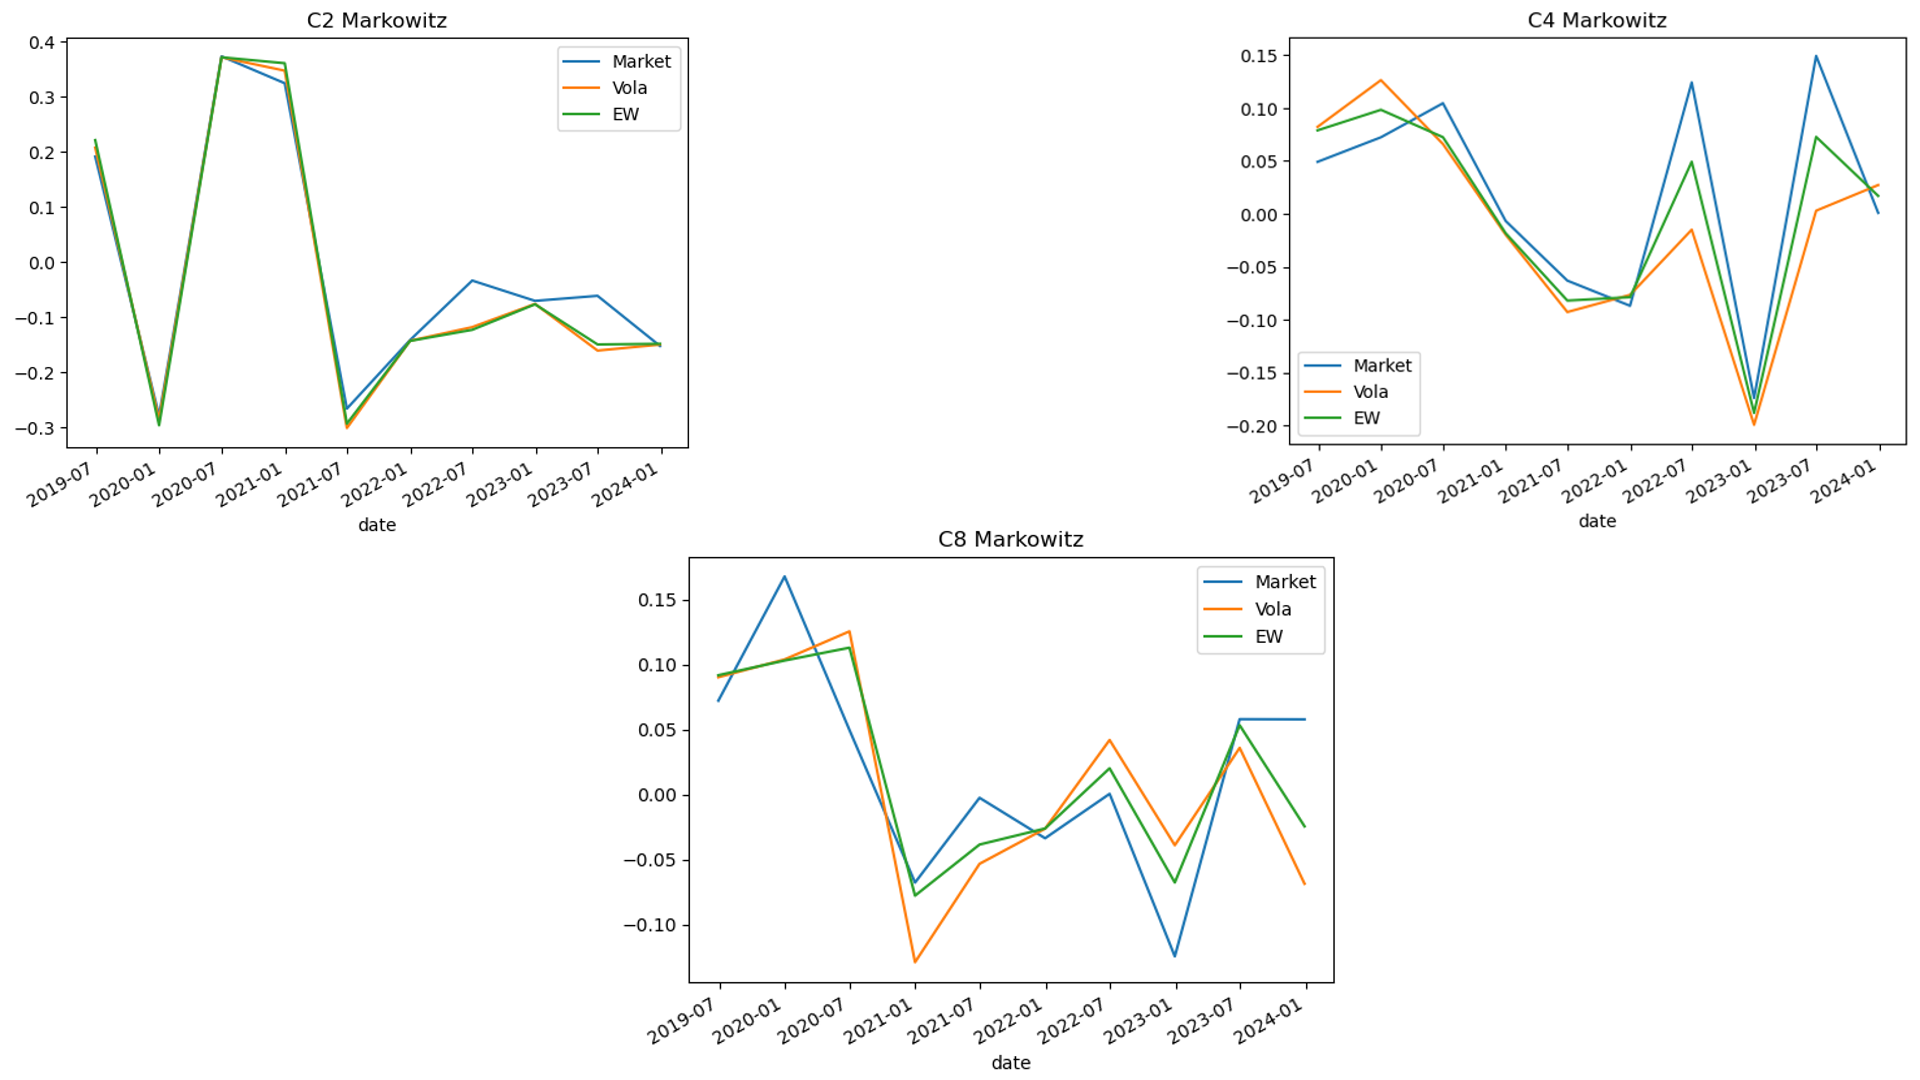
\includegraphics[width=10cm]{optimizado no acotado por cluster por tiempo.png}
        \caption{Error de seguimiento de portafolios con pesos optimizados con Markowitz pero no acotados, 
        con respecto al IPC S\&P/BMV según tipo de \textit{clustering} y \textit{benchmark} con respecto al tiempo}
    \end{figure}
\end{frame}

\begin{frame}{Resultados: Error de seguimiento en portafolio optimizado con Markowitz pero no acotado}
    \begin{figure}[htp]
        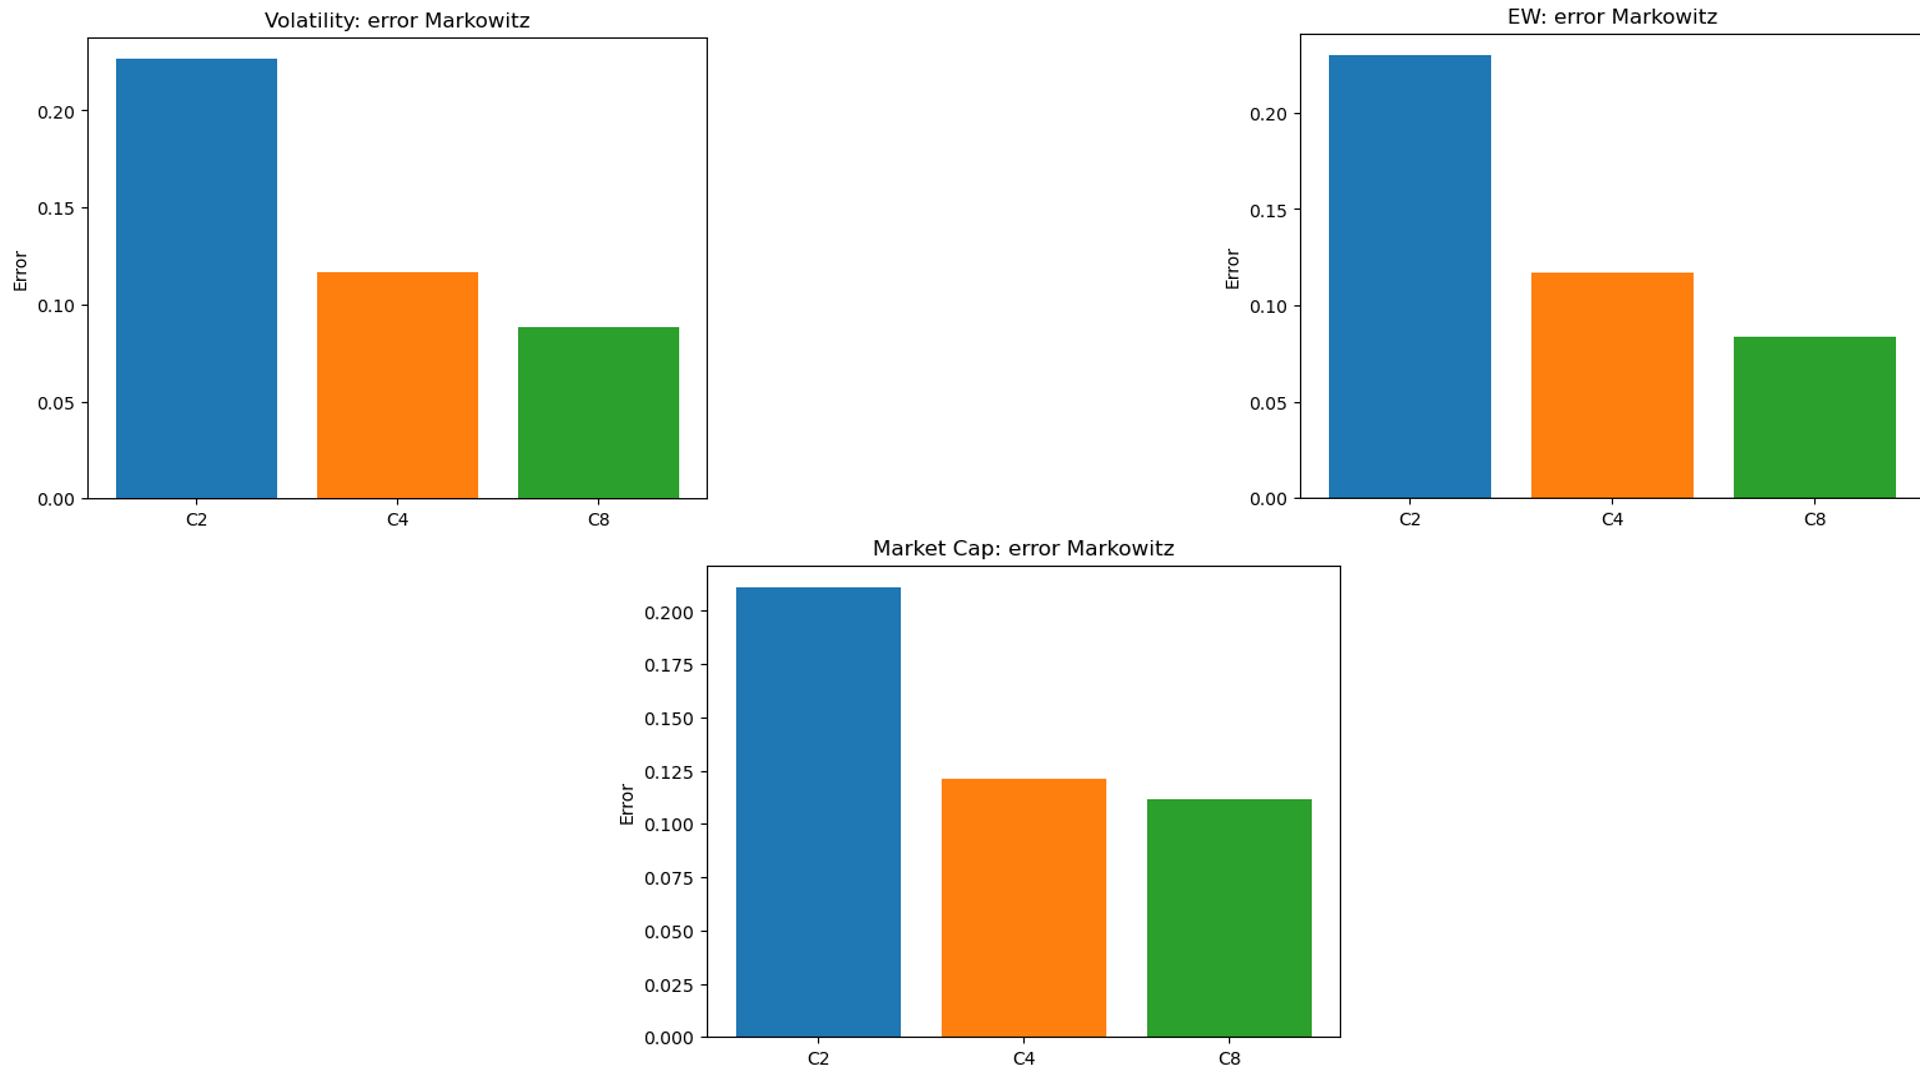
\includegraphics[width=10cm]{optimizado no acotado total por tipo.png}
        \caption{Error total de seguimiento de portafolios con pesos optimizados con Markowitz pero no acotados,
        con respecto al IPC S\&P/BMV según tipo de \textit{benchmark} y \textit{clustering}}
    \end{figure}
\end{frame}

\begin{frame}{Resultados: Error de seguimiento en portafolio optimizado con Markowitz pero no acotado}
    \begin{figure}[htp]
        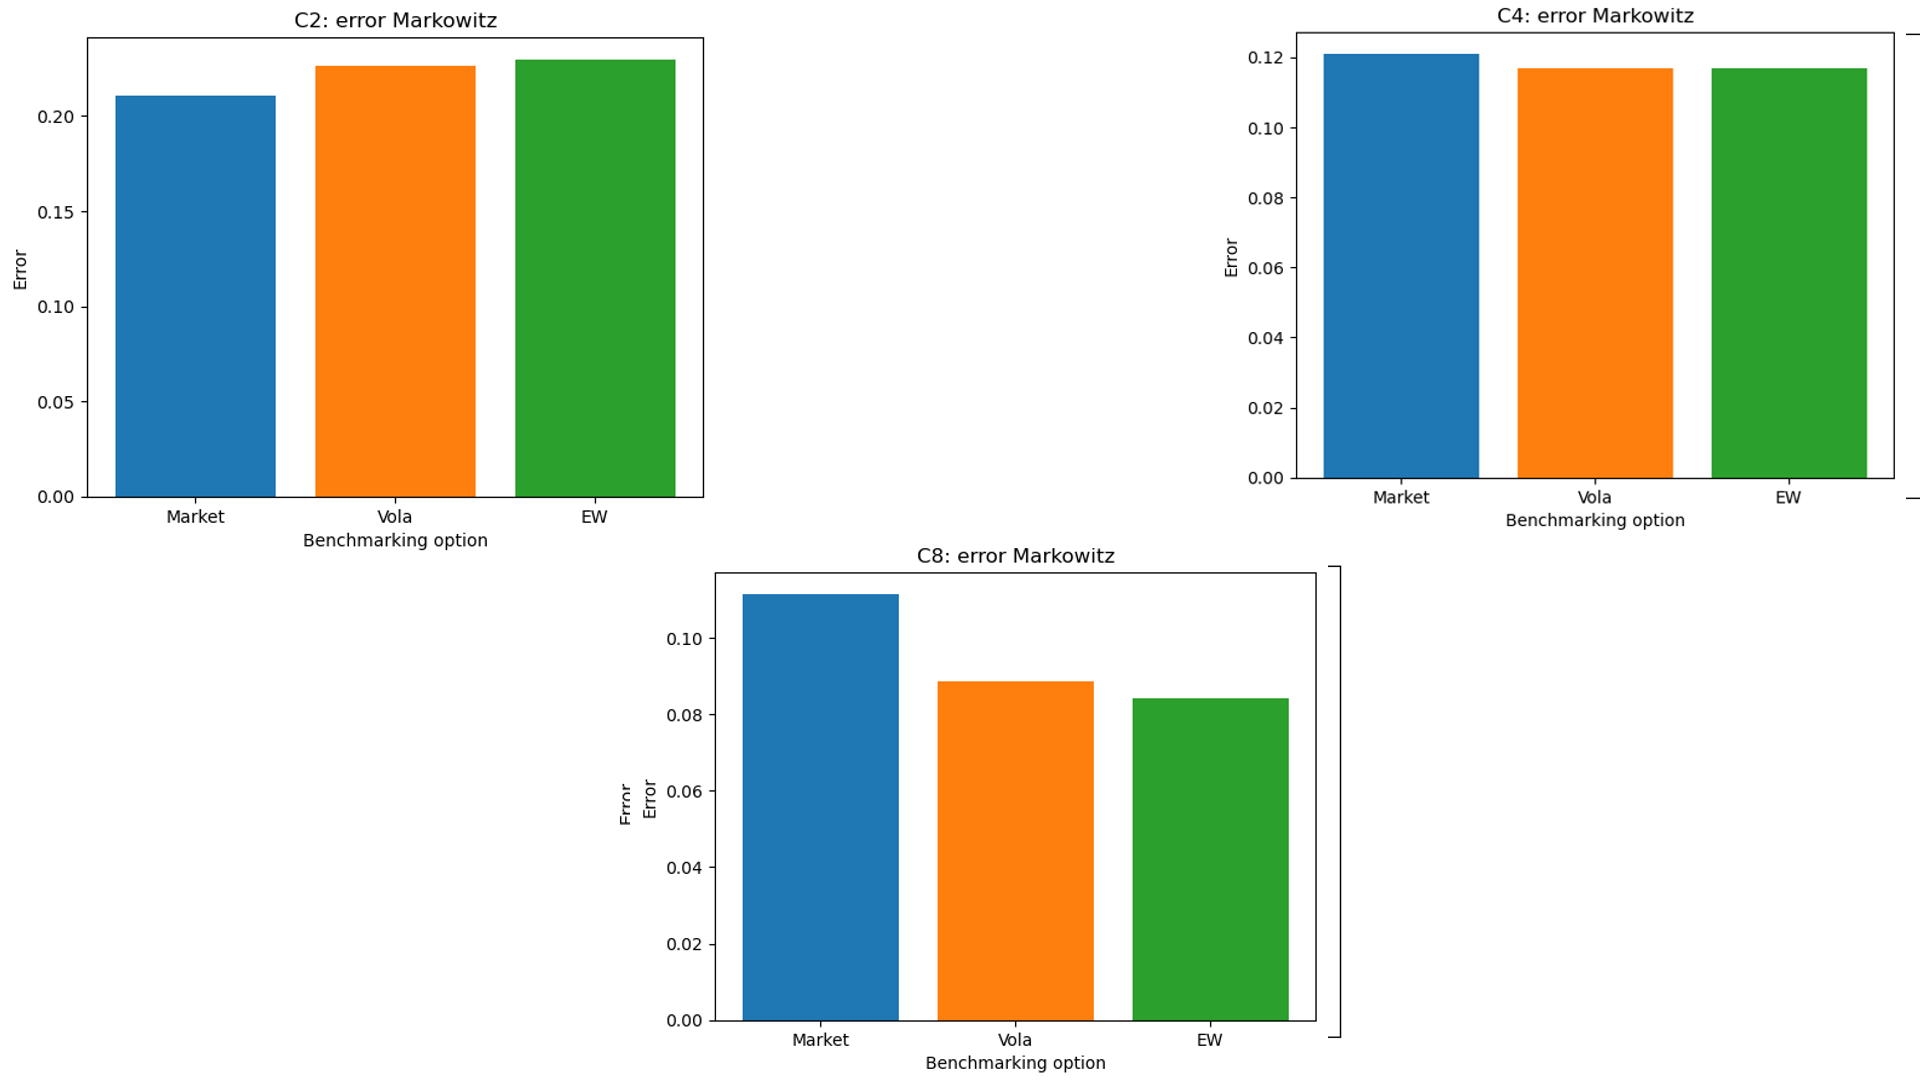
\includegraphics[width=10cm]{optimizado no acotado total por clusters.png}
        \caption{Error total de seguimiento de portafolios con pesos optimizados con Markowitz pero no acotados,
        con respecto al IPC S\&P/BMV según tipo de \textit{clustering} y \textit{benchmark}}
    \end{figure}
\end{frame}

\begin{frame}{Resultados: Error de seguimiento en portafolios \textit{benchmark} vs optimizado con Markowitz
     pero no acotado}
    \begin{figure}[htp]
        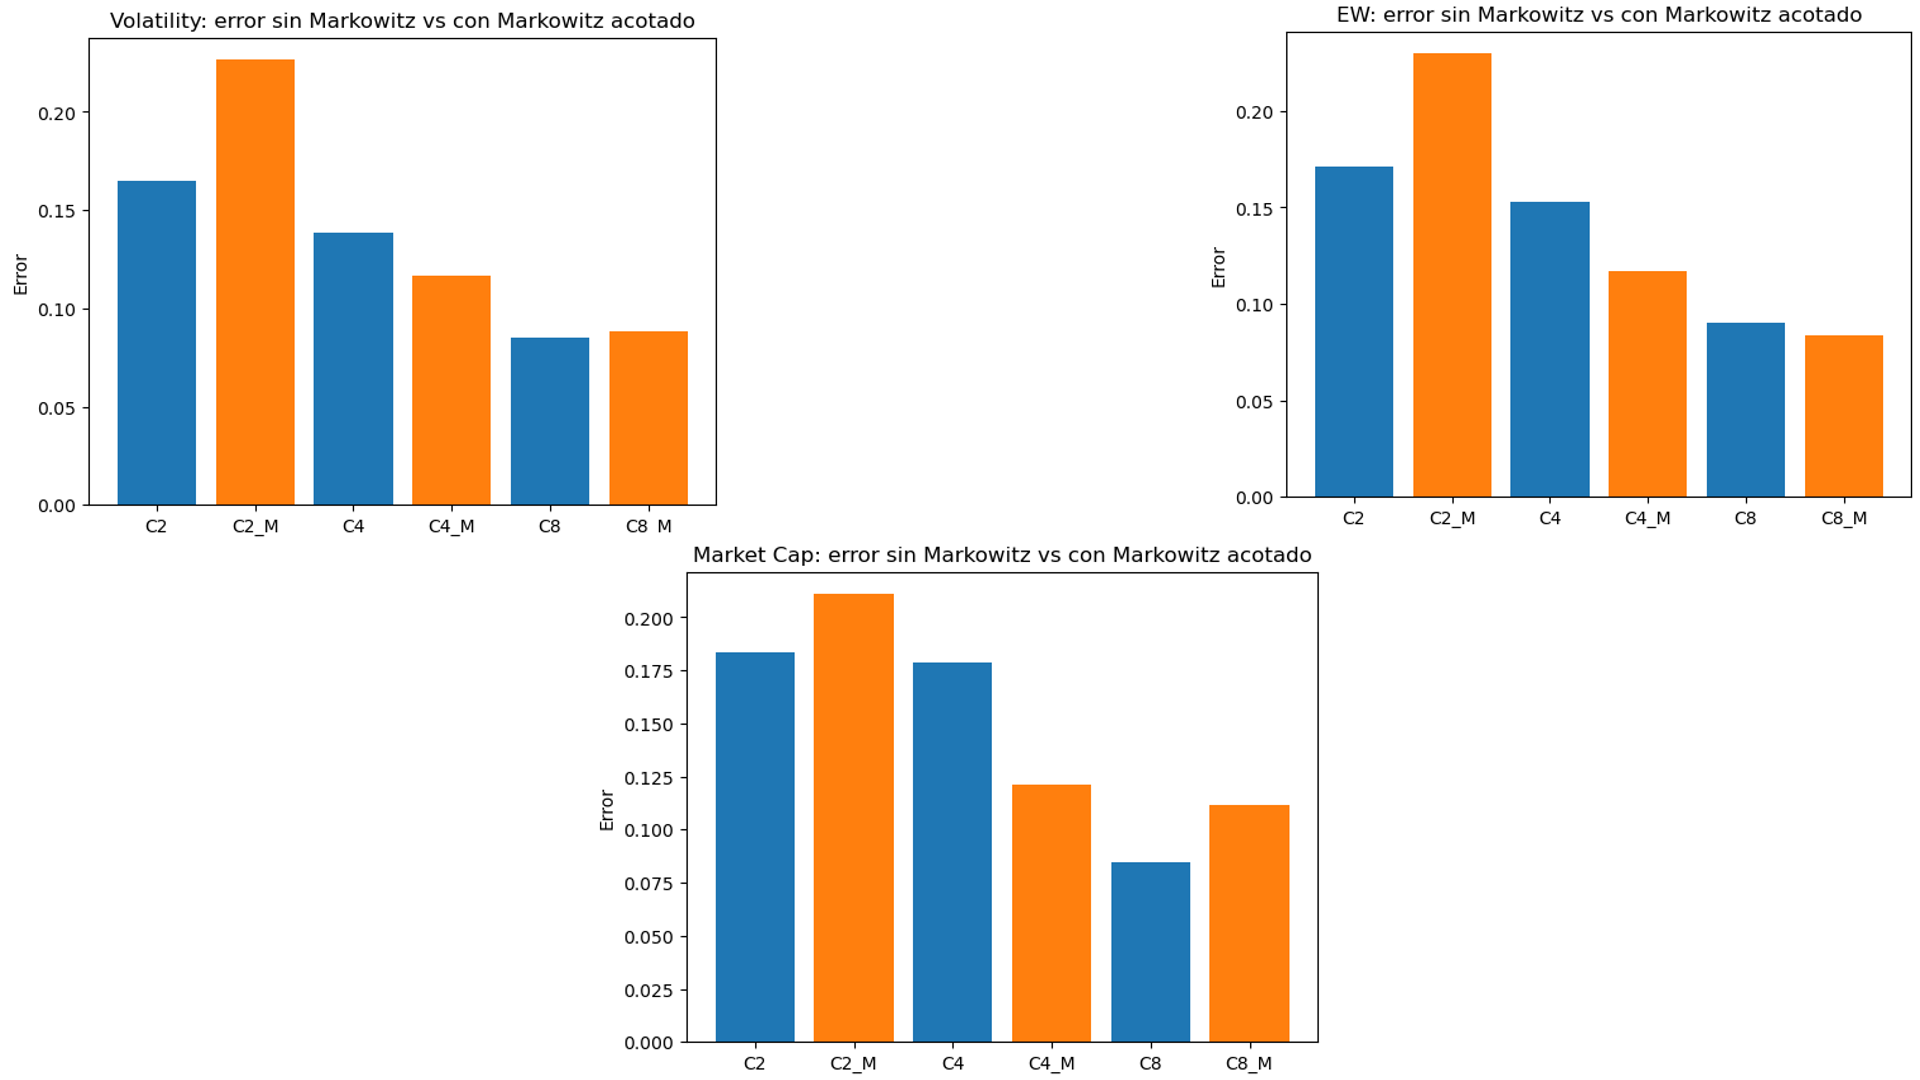
\includegraphics[width=10cm]{sin optimizar vs no acotado por tipo.png}
        \caption{Compraciones de errores totales de seguimiento de portafolios con pesos del \textit{benchmark} 
        vs optimizados con Markowitz pero no acotados, con respecto al IPC S\&P/BMV según tipo de 
        \textit{benchmark} y \textit{clustering}}
    \end{figure}
\end{frame}

\begin{frame}{Resultados: Error de seguimiento en portafolios \textit{benchmark} vs optimizado con Markowitz
     pero no acotado}
    \begin{figure}[htp]
        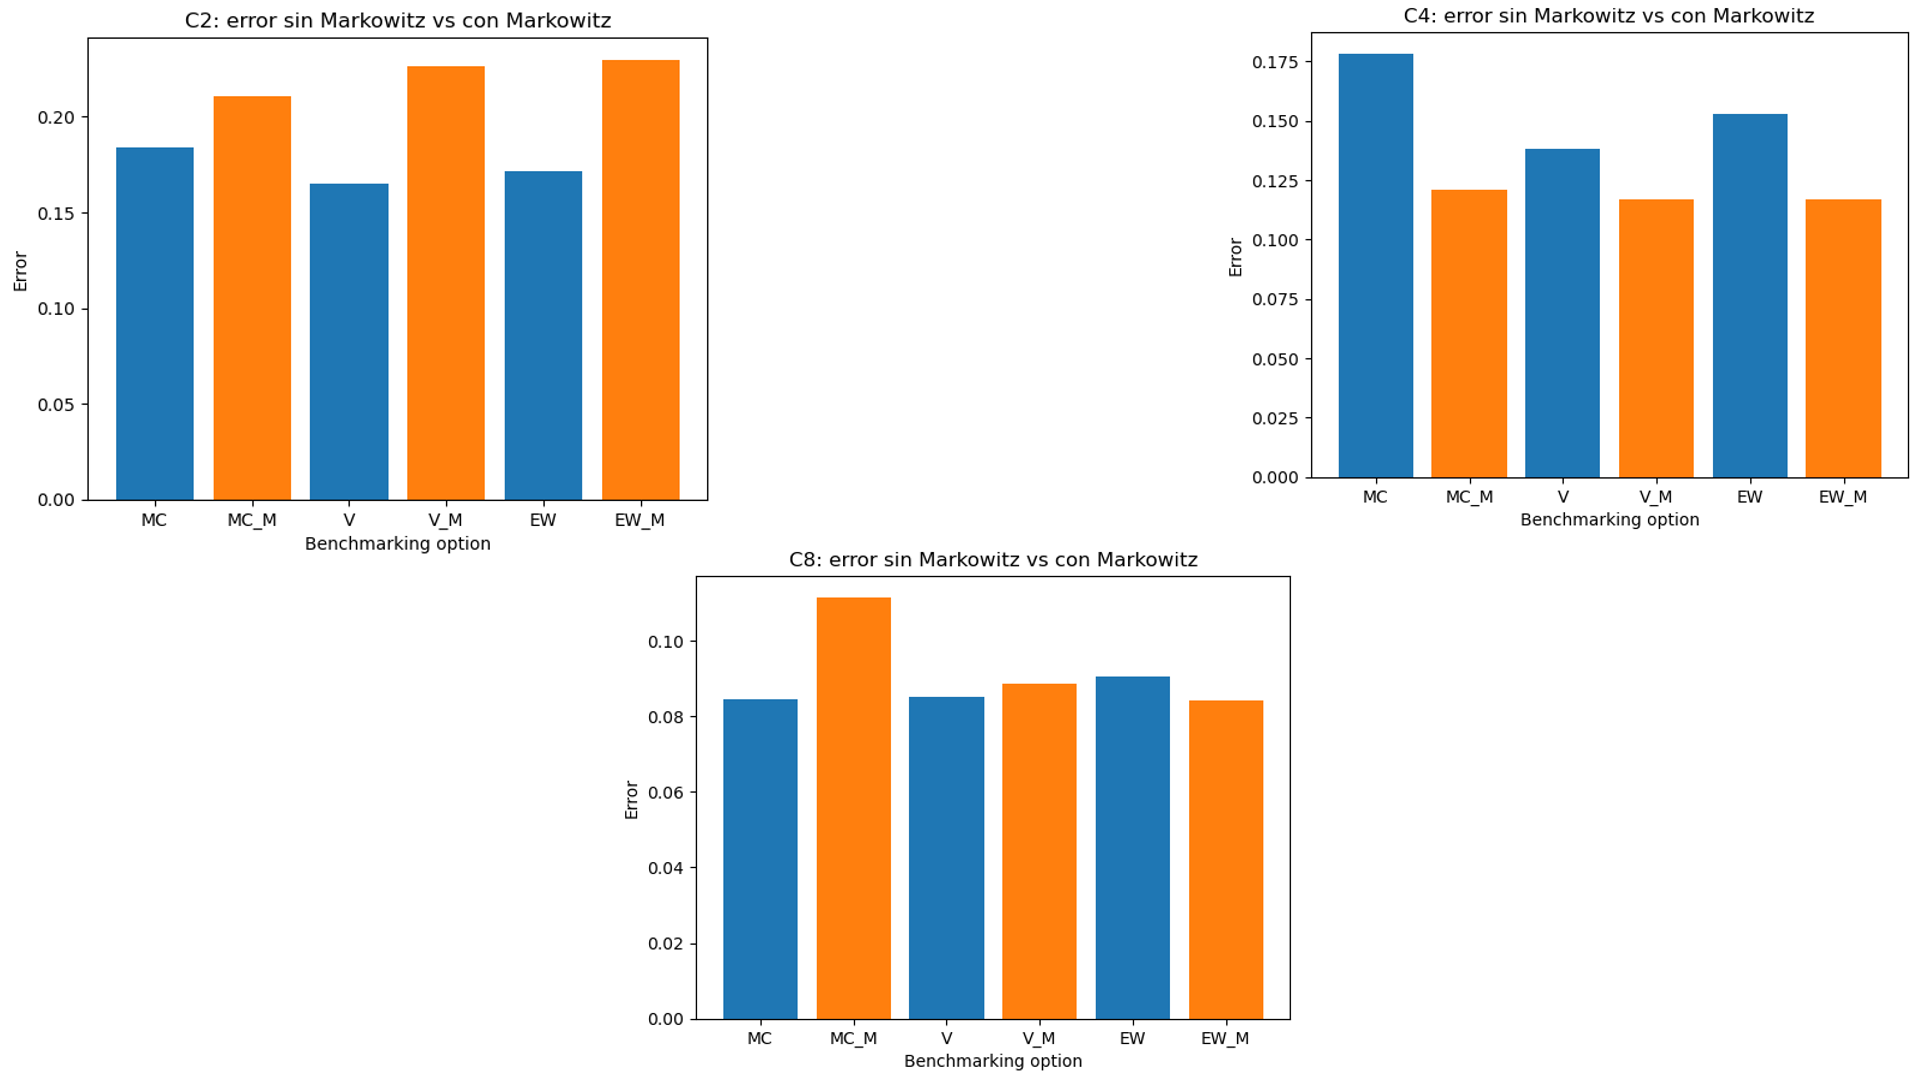
\includegraphics[width=10cm]{sin optimizar vs no acotado por cluster.png}
        \caption{Compraciones de errores totales de seguimiento de portafolios con pesos del \textit{benchmark} 
        vs optimizados con Markowitz pero no acotados, con respecto al IPC S\&P/BMV según tipo de 
        \textit{clustering} y \textit{benchmark}}
    \end{figure}
\end{frame}

\begin{frame}{Resultados: Turnover en portafolios optimizado con Markowitz pero no acotado}
    \begin{figure}[htp]
        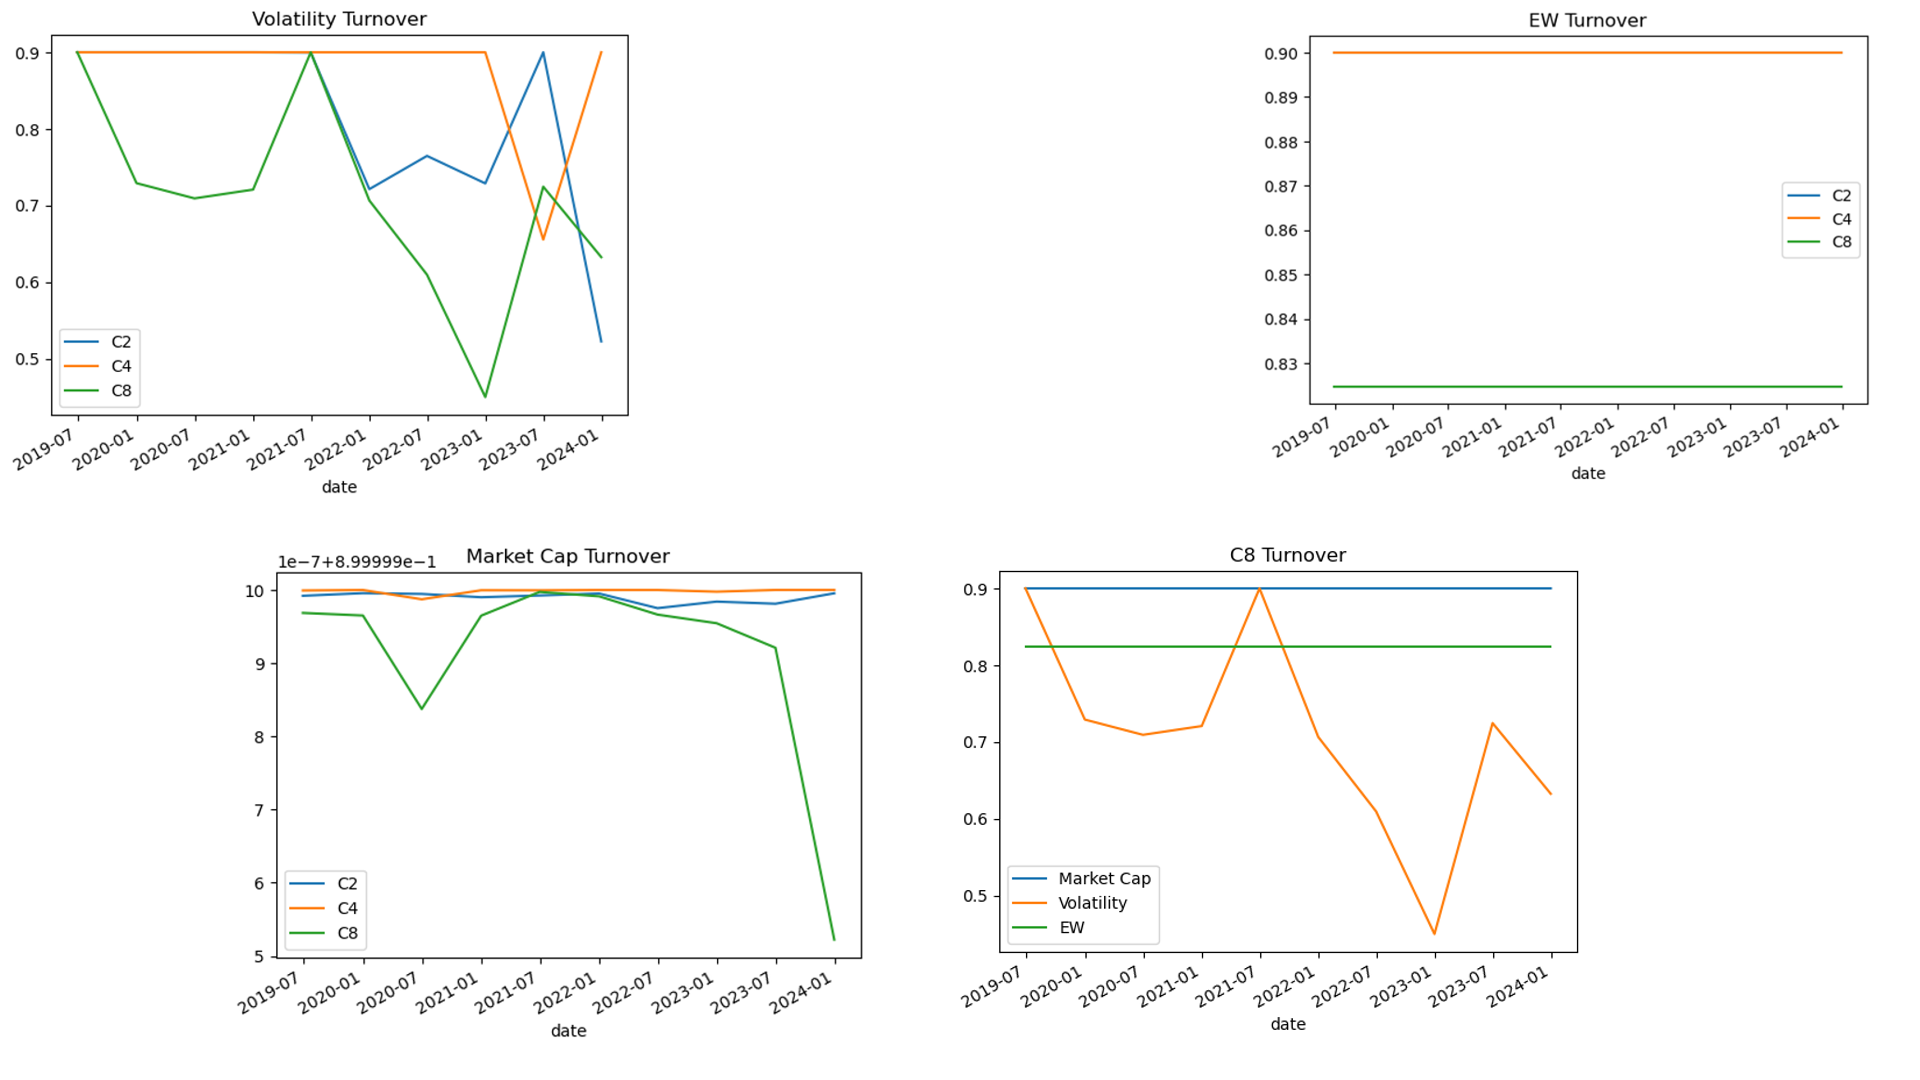
\includegraphics[width=10cm]{TUrnover por tipo por fecha.png}
        \caption{turnovers de los portafolios optimizados con Markowitz pero no acotados, con respecto al IPC 
        S\&P/BMV según el período}
    \end{figure}
\end{frame}

\begin{frame}{Resultados: Error de seguimiento en portafolios optimizados con Markowitz y acotados}
    \begin{figure}[htp]
        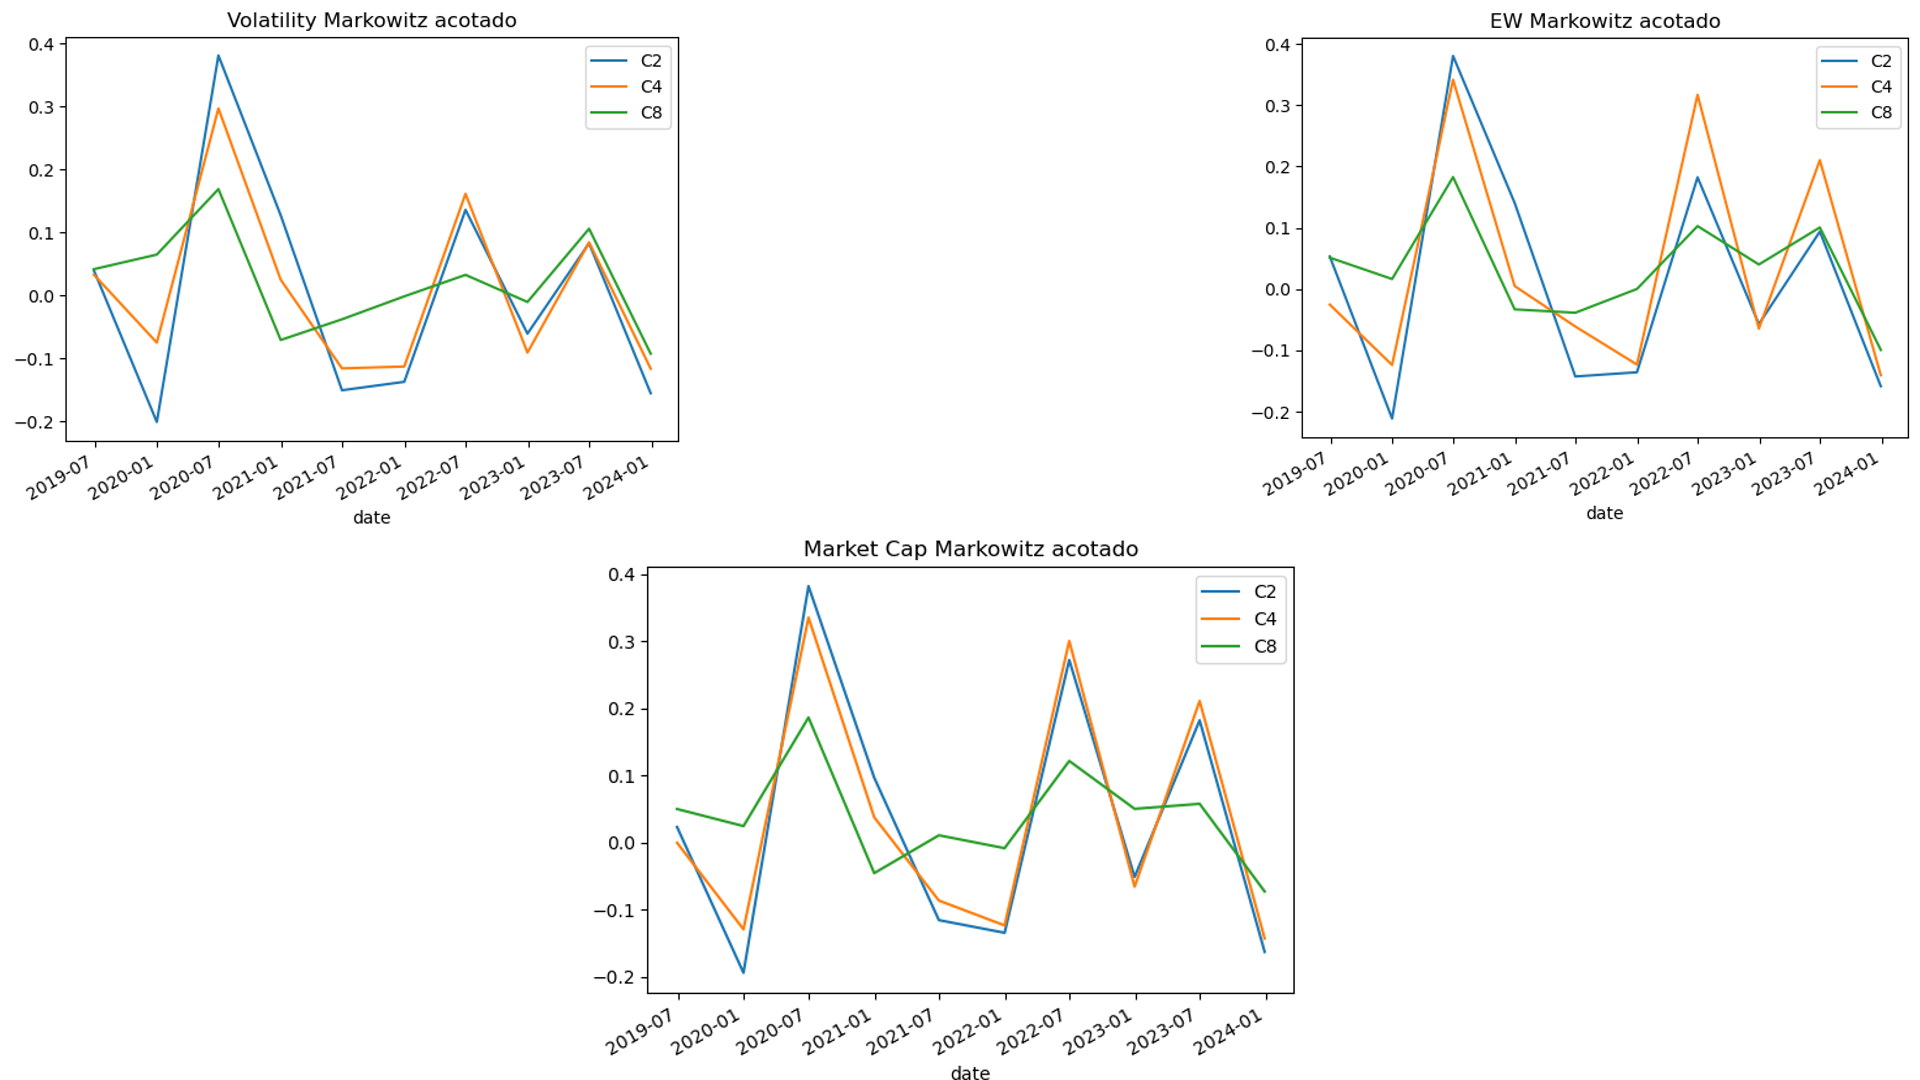
\includegraphics[width=10cm]{optimizado por tipo por tiempo.png}
        \caption{Error de seguimiento de portafolios optimizados con Markowitz y acotados con respecto al IPC 
        S\&P/BMV según tipo de \textit{benchmark} y \textit{clustering} con respecto al tiempo}
    \end{figure}
\end{frame}

\begin{frame}{Resultados: Error de seguimiento en portafolios optimizados con Markowitz y acotados}
    \begin{figure}[htp]
        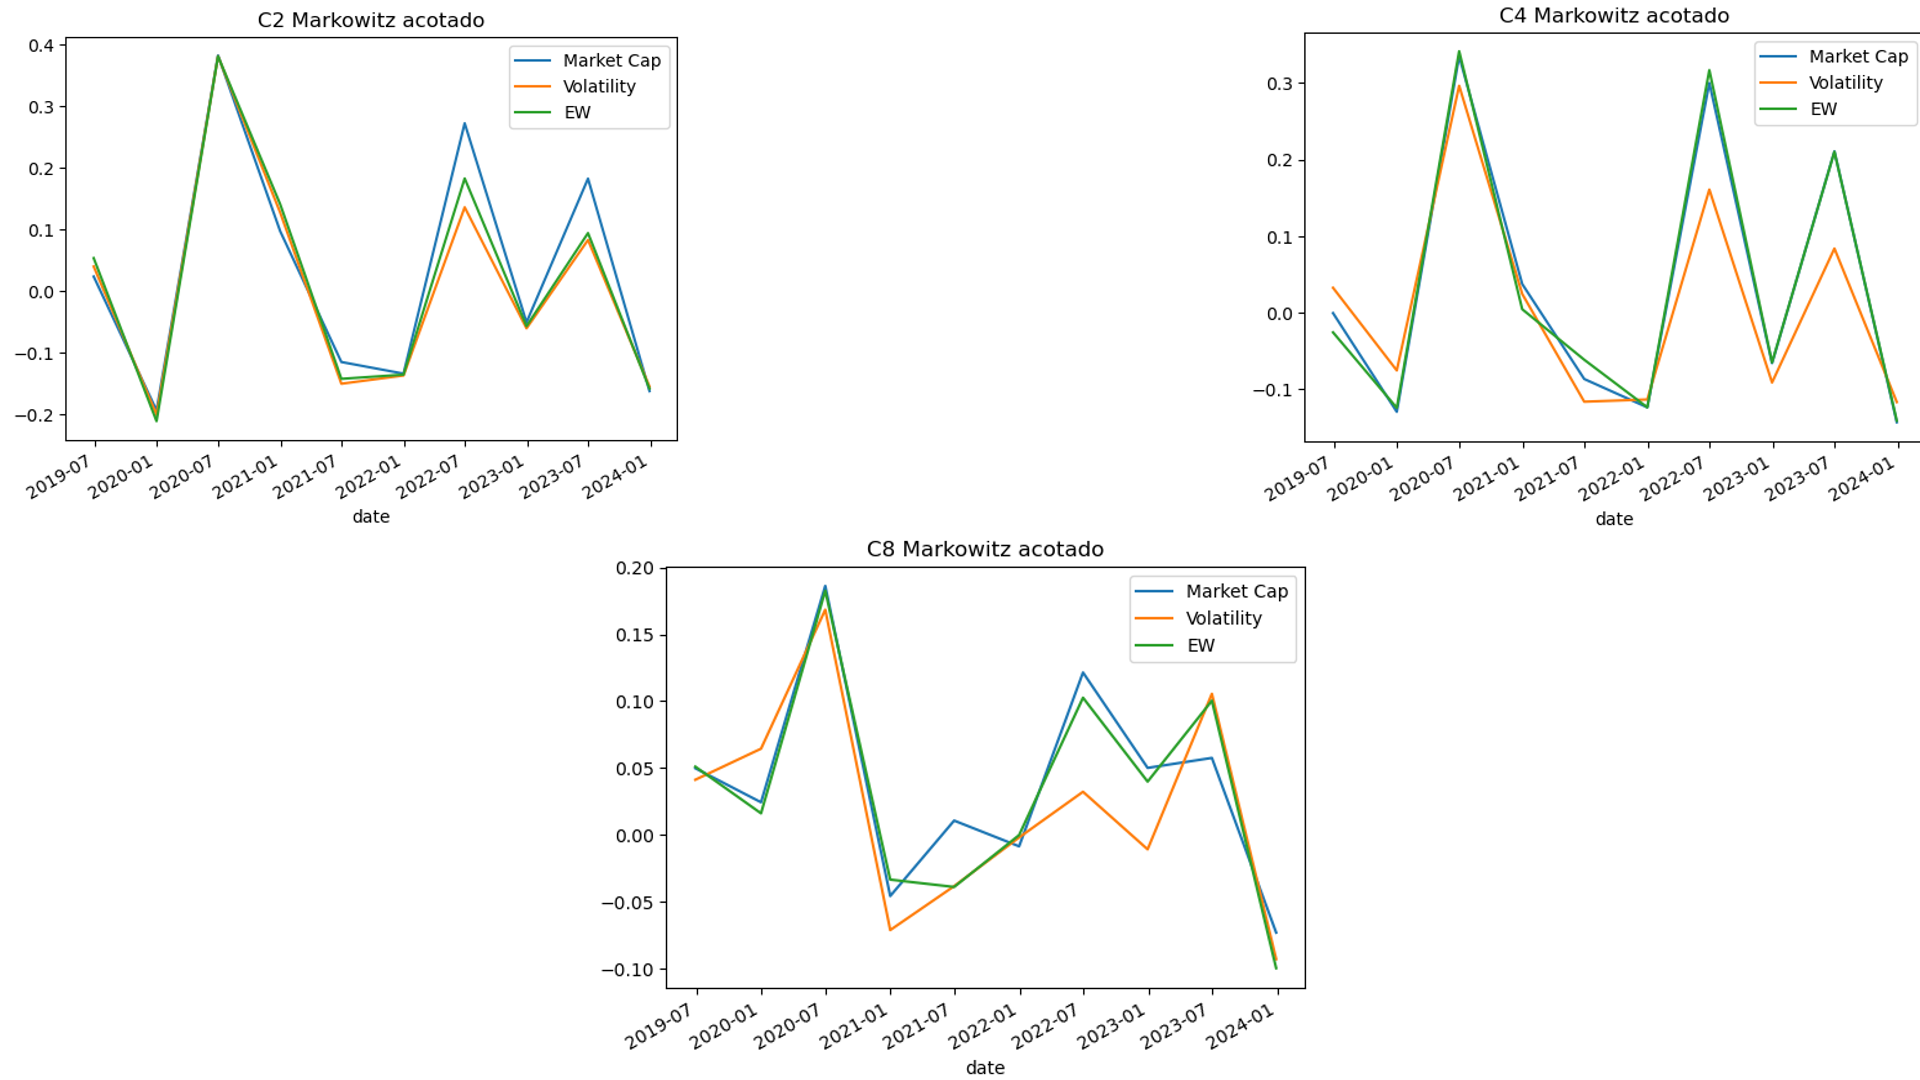
\includegraphics[width=10cm]{optimizado por cluster por tiempo.png}
        \caption{Error de seguimiento de portafolios optimizados con Markowitz y acotados con respecto al 
        IPC S\&P/BMV según tipo de \textit{clustering} y \textit{benchmark} con respecto al tiempo}
    \end{figure}
\end{frame}

\begin{frame}{Resultados: Error de seguimiento en portafolios de \textit{benchmarks} vs optimizados 
    con Markowitz y acotados}
    \begin{figure}[htp]
        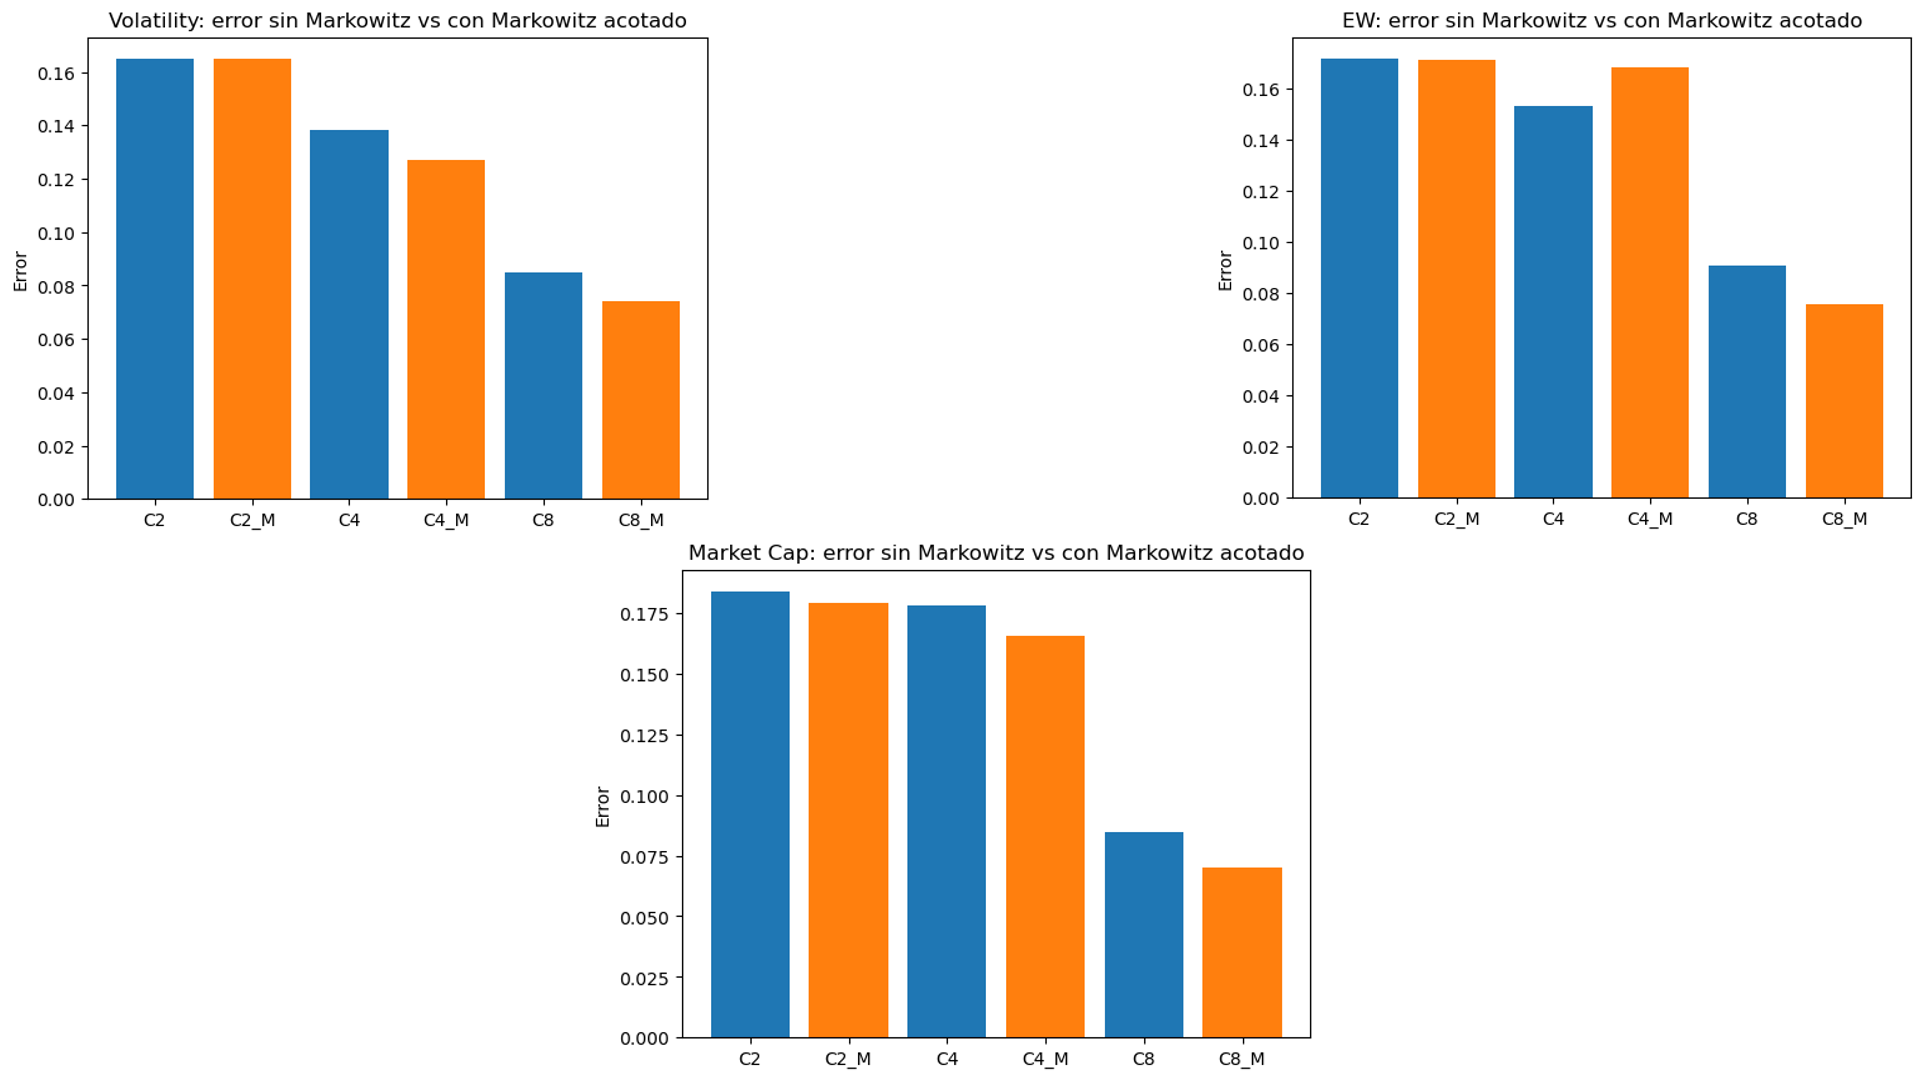
\includegraphics[width=10cm]{sin optimizar vs acotado por tipo.png}
        \caption{Comparación error de seguimiento de portafolios con pesos de \textit{benchmarks} vs 
        optimizados con Markowitz y acotados con respecto al IPC S\&P/BMV según tipo de \textit{benchmark}}
    \end{figure}
\end{frame}

\begin{frame}{Resultados: Error de seguimiento en portafolios de \textit{benchmarks} vs optimizados 
    con Markowitz y acotados}
    \begin{figure}[htp]
        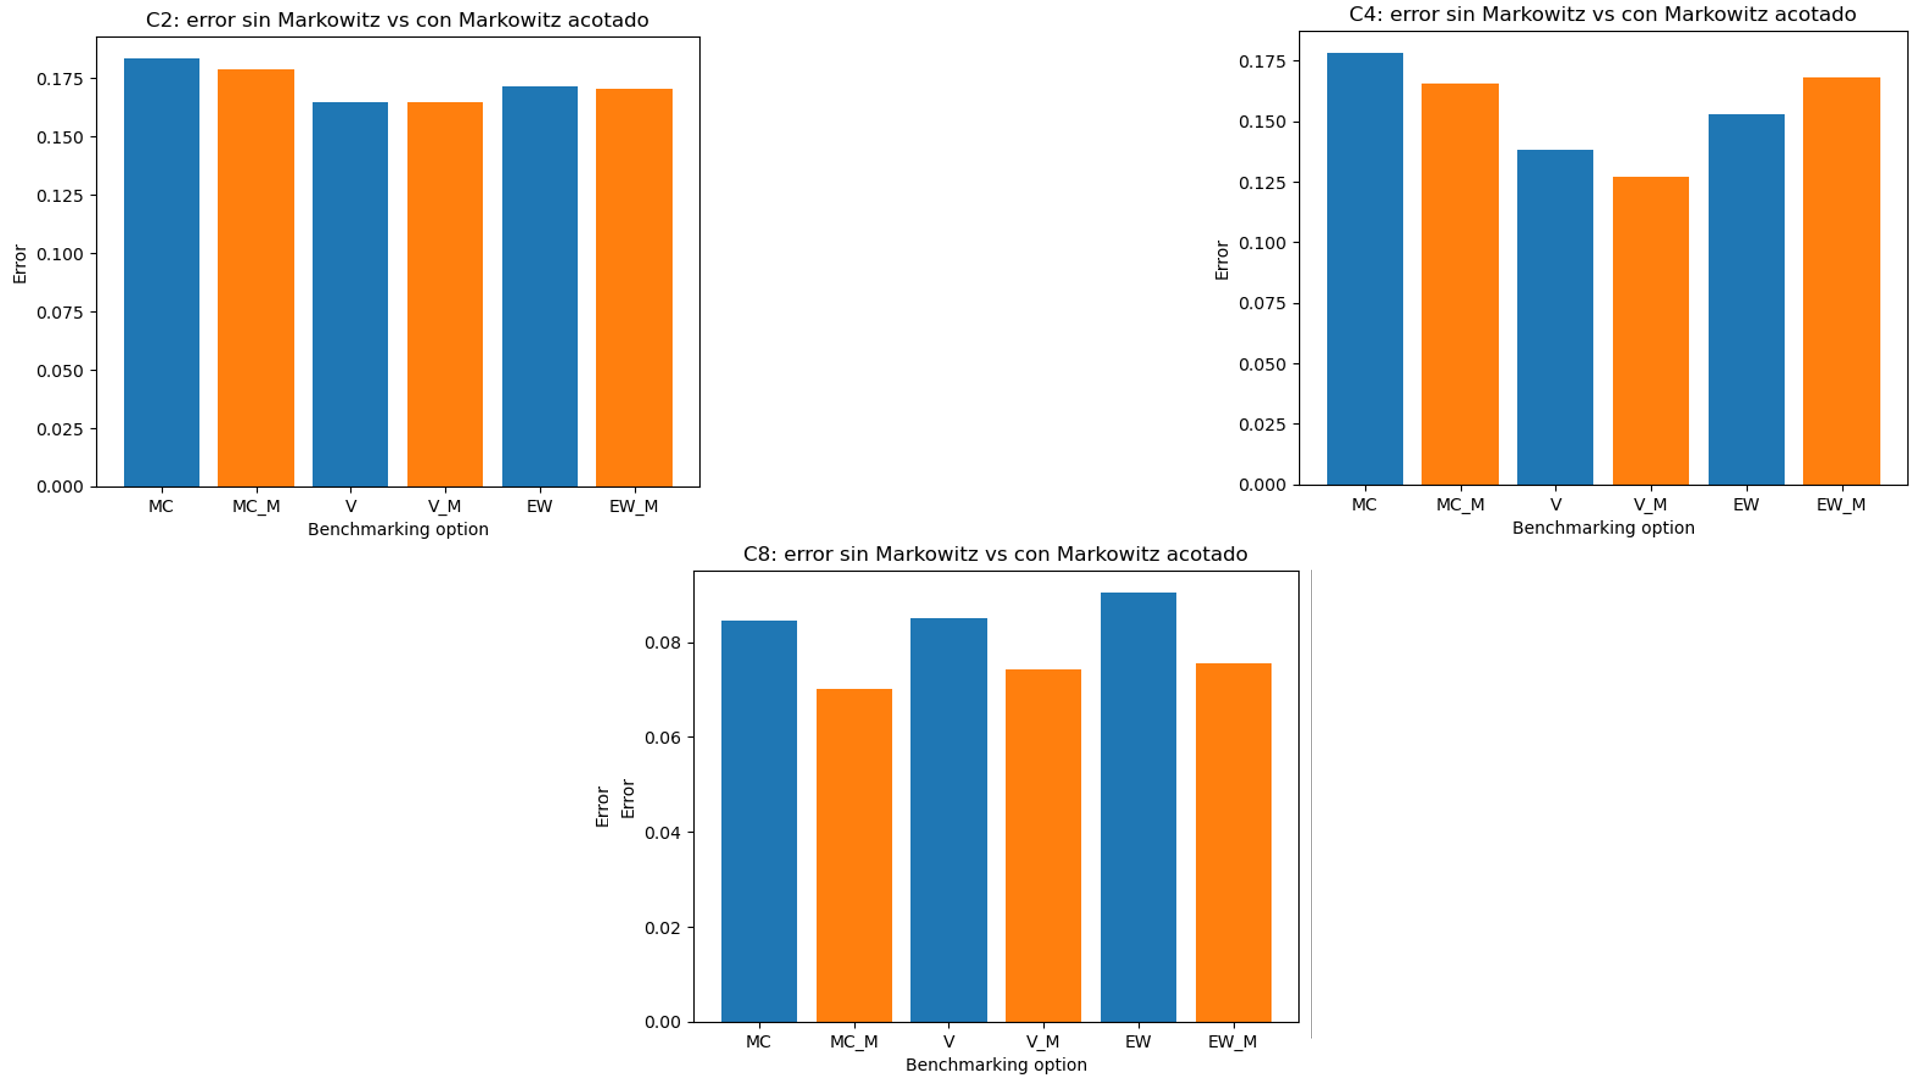
\includegraphics[width=10cm]{sin optimizar vs acotado por cluster.png}
        \caption{Comparación error de seguimiento de portafolios con pesos de \textit{benchmarks} vs 
        optimizados con Markowitz y acotados con respecto al IPC S\&P/BMV según tipo de \textit{clustering}}
    \end{figure}
\end{frame}

\begin{frame}{Resultados: Comparación de error de seguimiento entre todos}
    \begin{figure}[htp]
        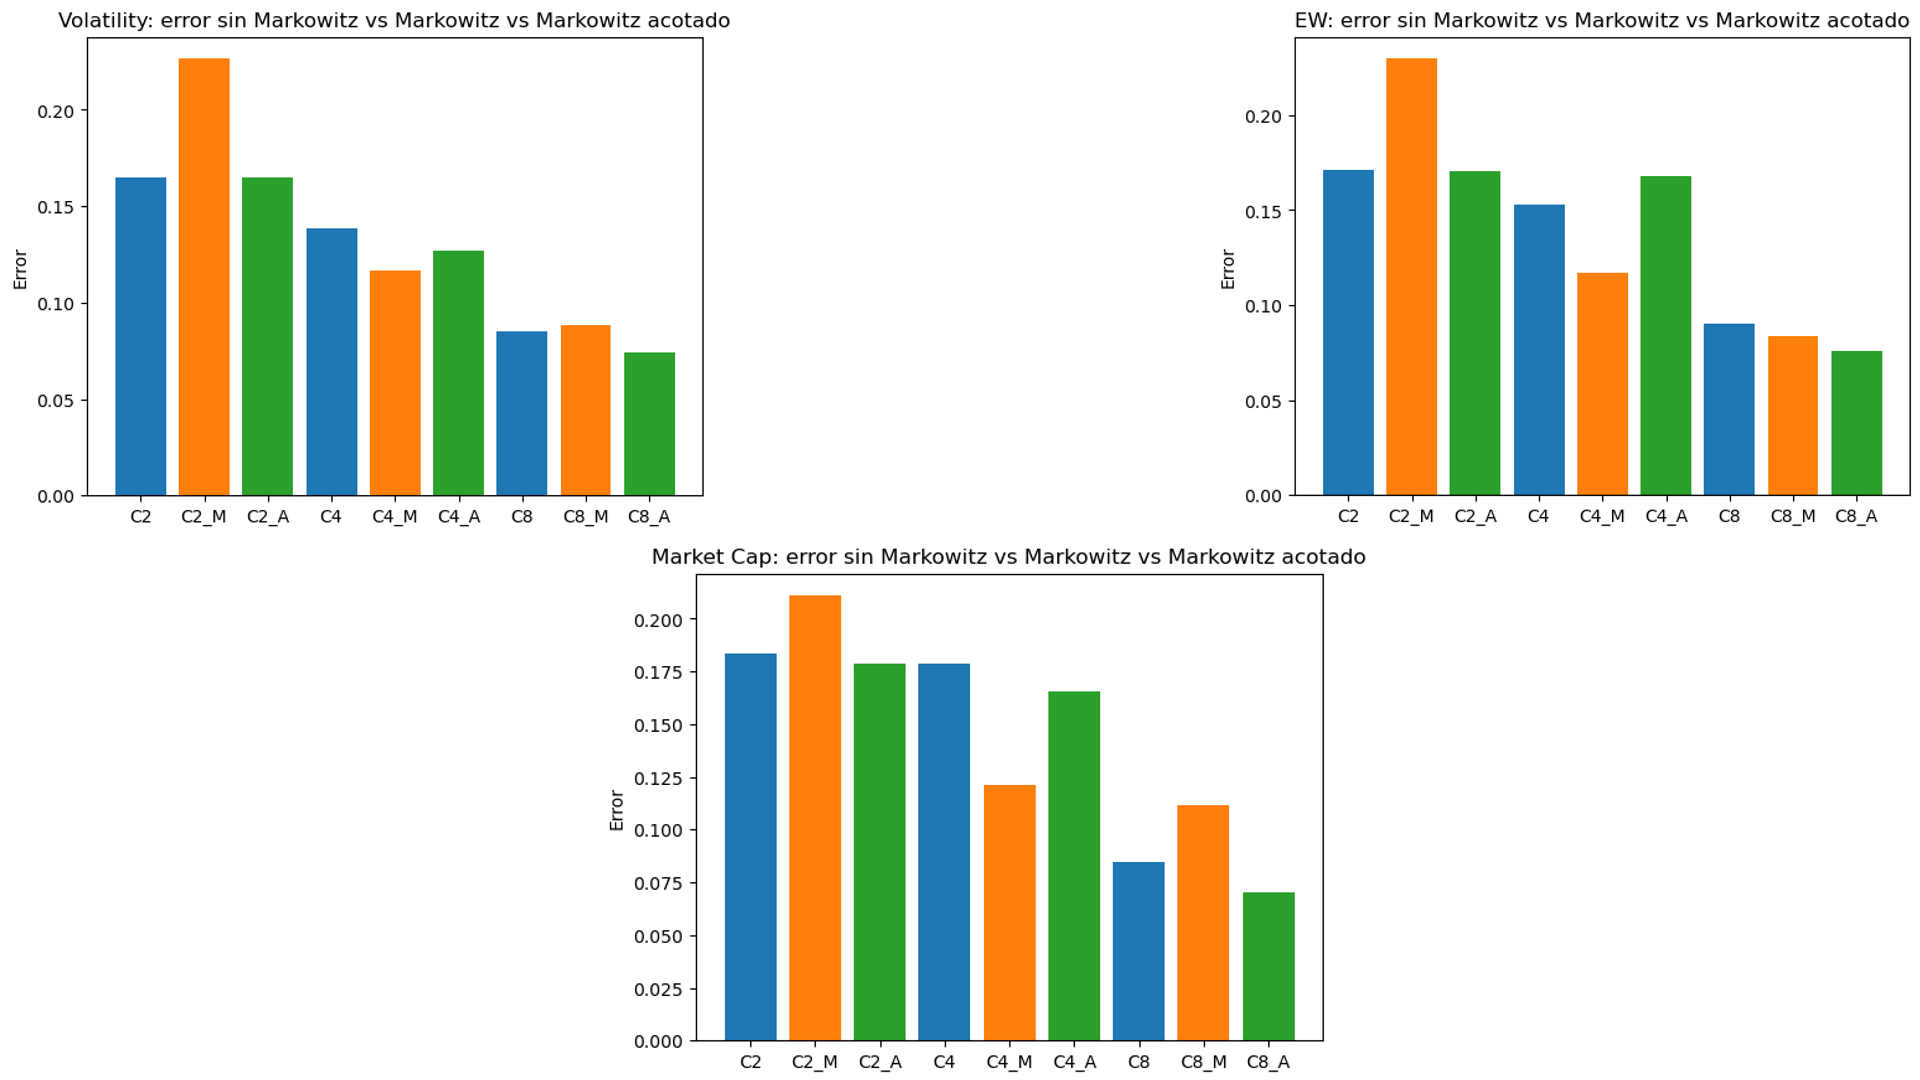
\includegraphics[width=10cm]{todos vs todos por tipo.png}
        \caption{Comparación error de seguimiento de portafolios con pesos de \textit{benchmarks} 
        vs optimizados con Markowitz y no acotados vs optimizados con Markowitz y acotados con respecto 
        al IPC S\&P/BMV según tipo de \textit{benchmark}}
    \end{figure}
\end{frame}

\begin{frame}{Resultados: Comparación de error de seguimiento entre todos}
    \begin{figure}[htp]
        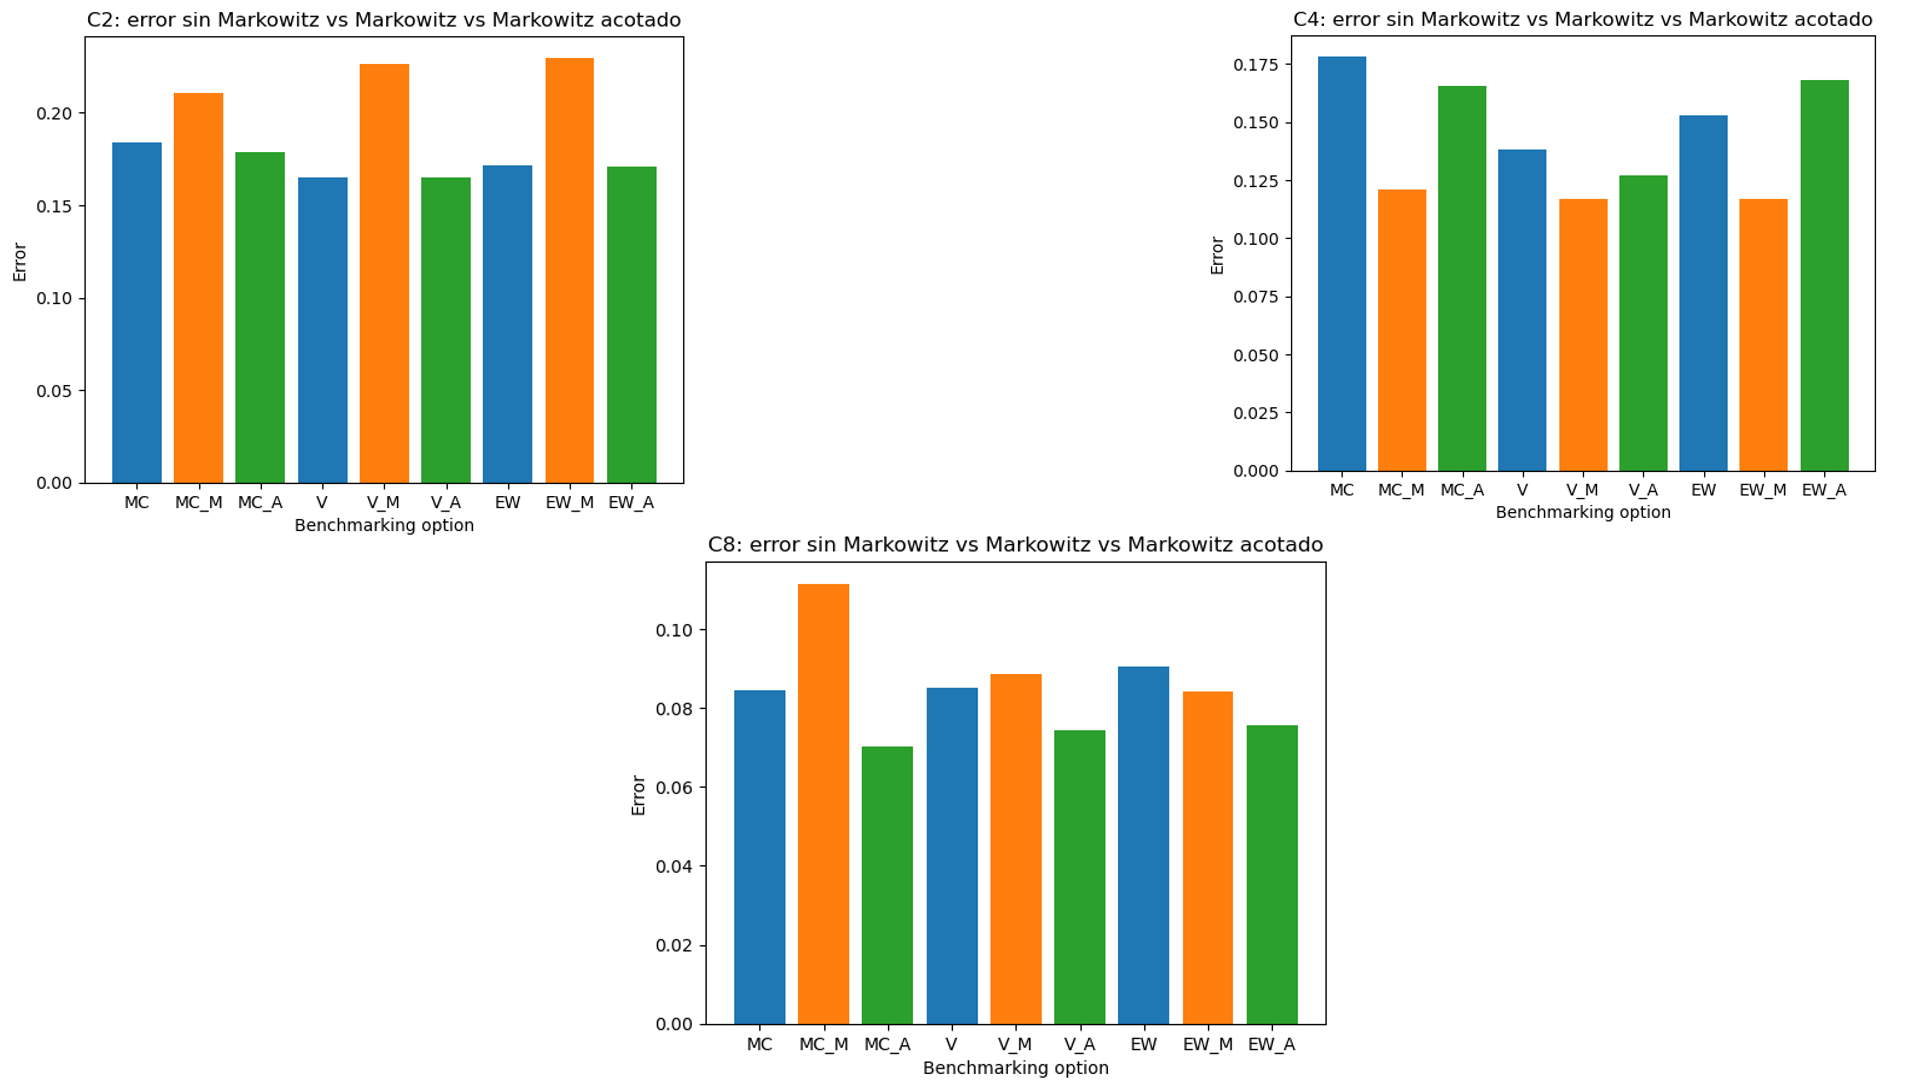
\includegraphics[width=10cm]{todos vs todos por cluster.png}
        \caption{Comparación error de seguimiento de portafolios con pesos de \textit{benchmarks} 
        vs optimizados con Markowitz y no acotados vs optimizados con Markowitz y acotados con 
        respecto al IPC S\&P/BMV según tipo de \textit{clustering}}
    \end{figure}
\end{frame}

\begin{frame}{Resultados: Comparación de error de seguimiento entre todos}
    \begin{figure}[htp]
        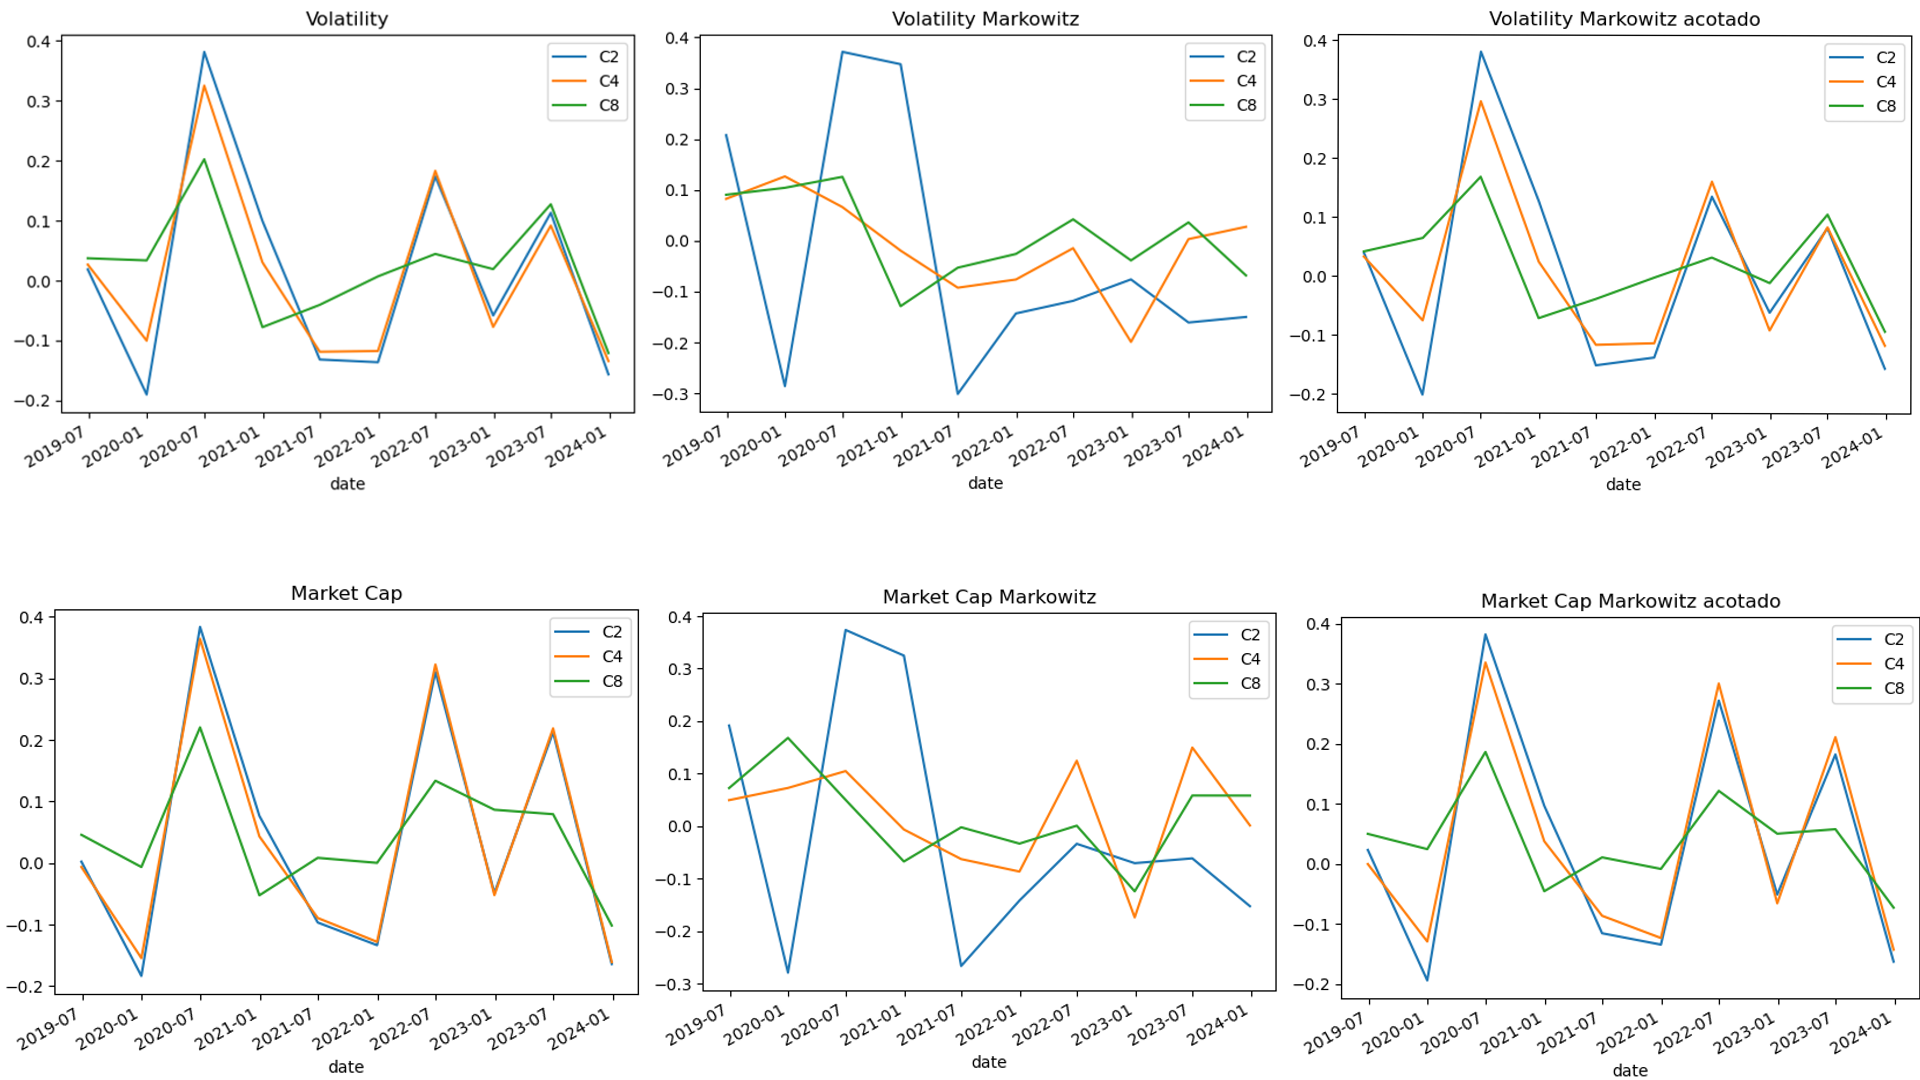
\includegraphics[width=10cm]{Vola Market todos.png}
        \caption{Comparación error de seguimiento de portafolios con pesos de 
        \textit{benchmarks} vs optimizados con Markowitz y no acotados vs optimizados 
        con Markowitz y acotados con respecto al IPC S\&P/BMV para la volatilidad (arriba)
         y capitalización de mercado (abajo)}
    \end{figure}
\end{frame}
\begin{frame}{Resultados: Comparación de error de seguimiento entre todos}
    \begin{figure}[htp]
        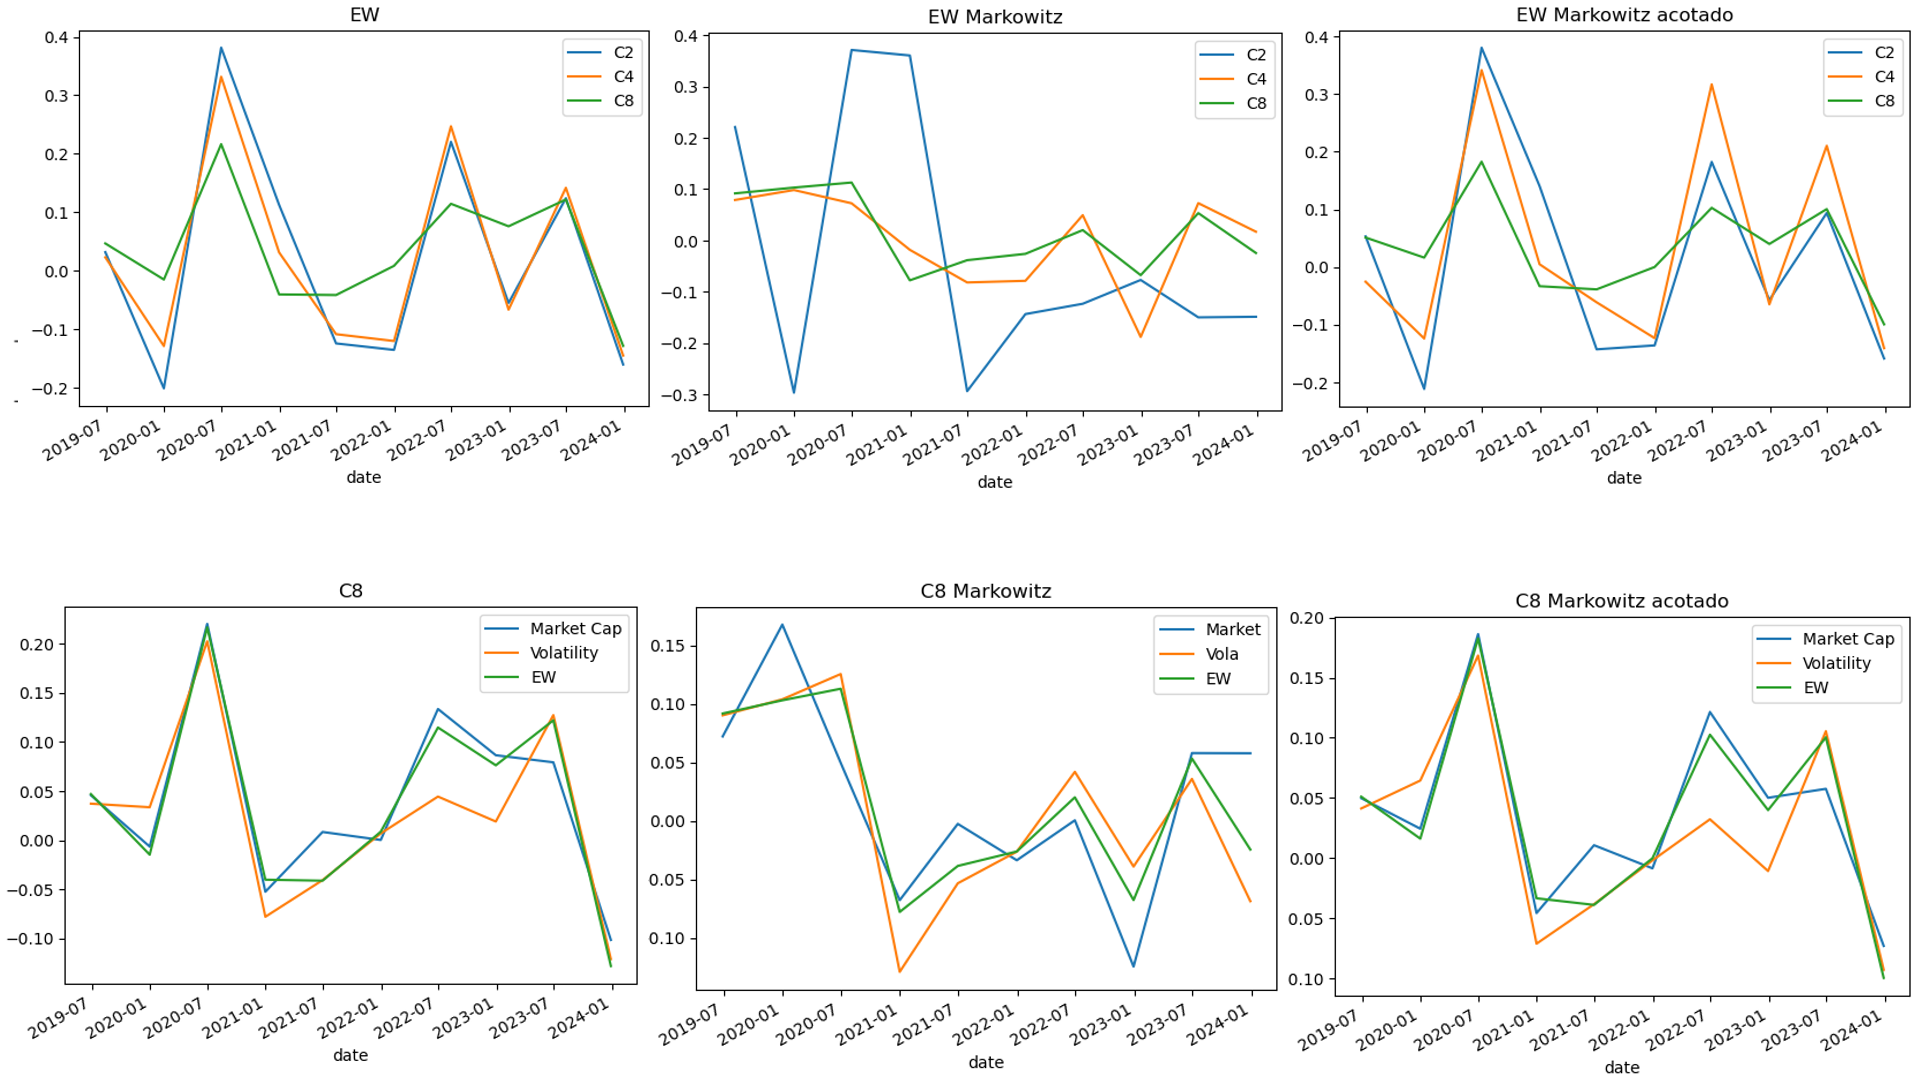
\includegraphics[width=10cm]{EW C8 todos.png}
        \caption{Comparación error de seguimiento de portafolios con pesos de \textit{benchmarks}
        vs optimizados con Markowitz y no acotados vs optimizados con Markowitz y acotados con 
        respecto al IPC S\&P/BMV para \textit{Equally Weighted} (arriba) y \textit{clustering} con 8 (abajo)}
    \end{figure}
\end{frame}

\section{Conclusiones}
\begin{frame}{Conclusiones}
    \begin{itemize}
        \item No se llegó a un portafolio con un error de seguimiento significativo $\leq 5\%$.
        \item No hubo una consitencia clara en los resultados para sugerir la optimilidad de algún portafolio o cantidad de clústeres.
        \item A pesar de haber poseído limitantes semejantes a otros trabajos similares, los resultados no son consistentes con estos.
        \item Se pudieron haber evalúado otras métricas y haber probado la optimización con otras cotas.
    \end{itemize}
\end{frame}

\begin{frame}{Conclusiones}
    Donde yacen las diferencias es en las características propias del mercado mexicano:
    \begin{itemize}
        \item Pocas emisoras en el IPC.
        \item Concentración sectorial.
        \item Particularidades en la marcoeconomía.
        \item Los eventos que se traducen en riesgo sistémico.
        \item En general no toma en cuenta el valor, crecimiento, momentum, tamaño o calidad de mercado.
    \end{itemize}
\end{frame}
%------------------------------------------------
\section{Referencias}
%------------------------------------------------

\begin{frame}{Referencias (1/3)}
    \begin{enumerate}
        \def\labelenumi{\arabic{enumi}.}
        \item
        Gharanchaei, M. K., Panda, P. P. (2024). \emph{Constructing and
        investment fund thourg stock clustering and integer programming}.
        Journal of Advancements in Applied Business Research.
        \item
        Markowitz, H. (1952). \emph{Portfolio selection}. JSTOR. (pp 77- 91).
        \item
        Wolsey Laurence, A. (1998). Formulations. \emph{Integer Programming}.
        (pp. 1-18). Wiley Interscience.
        \item
        Bertsimas, D., Darnell, C., Soucy, R., (1998). \emph{Portfolio construction
        through mixed integer programming}. MIT.
        \item
        Kuhn, C. C. N., Calbert, G., Garanovich, I. L., Weir, T., (2023).
        \emph{Integer linear programming supporting portfolio design.}
        Elsevier.
        \item
        Anderson, R. M., Bianachi, S. W., Goldberg, L. R. (2011). \emph{Will
        My Risk Parity Strategy Outperform?} Berkeley.
        \item
        Baker, M., Bradley, B., Wurgler, J\emph{. Benchmarks as Limits to
        Arbitrage: Understanding the Low-Volatility Anomaly}. Financial
        Analysts Journal.
    \end{enumerate}
\end{frame}

\begin{frame}{Referencias (2/3)}
    \begin{enumerate}
        \item
        Koumou, G. B. (2020). \emph{Diversification and portfolio theory: a
        review}. Swiss Society for Financial Market Research.
        \item
        Knutzen, S., Retterholt, J., (2015). \emph{Performance of risk-based
        asset allocation strategies} {[}tesis master, Copenhagen Business
        School{]}.
        \item
        Choueifaty, Y., Coignard, Y. (2008). \emph{Toward Maximum
        Diversification}. The Journal of Portfolio Management.
        \item
        Reed, T; Muñoz Moreno, R. (febrero 23, 2023). \emph{How the Federal Economic
        Competition Commission fights for workers and consumers in Mexico}.
        World Bank.
        \item
        Chow, T., Hsu, J., Kalesnik, V., Little, B. (2011). \emph{A Survey of
        Alternative Equity Index Strategies.} Financial Analysts Journal.
\end{enumerate}
\end{frame}

\begin{frame}{Referencias (3/3)}
    \begin{enumerate}
        \item 
        Bacaria Colom, Jordi (2018). \textit{La nueva presidencia de México: entre la incertidumbre y la esperanza}. Barcelona Center for international affairs.
        \item 
        INEGI (2020). \textit{Economía y sectores productivos}. [Base de datos]
        \item 
        INEGI (2021). \textit{Economía y sectores productivos}. [Base de datos]
        \item
        S\&P Dow Jones Indices. (31 marzo 2025). S\&P/BMV IPC: \emph{Constituents Export}. {[}Base de datos{]}.
        \item
        Sánchez Deanny (octubre 6, 2023). Antitrust in Mexico: Perspectives,
        challenges, and opportunities.
    \end{enumerate}
\end{frame}
%------------------------------------------------

\begin{frame}
    \Huge{\centerline{\textbf{Gracias $<3$}}}
\end{frame}

%----------------------------------------------------------------------------------------

\end{document}